\documentclass[twoside]{book}

% Packages required by doxygen
\usepackage{fixltx2e}
\usepackage{calc}
\usepackage{doxygen}
\usepackage[export]{adjustbox} % also loads graphicx
\usepackage{graphicx}
\usepackage[utf8]{inputenc}
\usepackage{makeidx}
\usepackage{multicol}
\usepackage{multirow}
\PassOptionsToPackage{warn}{textcomp}
\usepackage{textcomp}
\usepackage[nointegrals]{wasysym}
\usepackage[table]{xcolor}

% Font selection
\usepackage[T1]{fontenc}
\usepackage[scaled=.90]{helvet}
\usepackage{courier}
\usepackage{amssymb}
\usepackage{sectsty}
\renewcommand{\familydefault}{\sfdefault}
\allsectionsfont{%
  \fontseries{bc}\selectfont%
  \color{darkgray}%
}
\renewcommand{\DoxyLabelFont}{%
  \fontseries{bc}\selectfont%
  \color{darkgray}%
}
\newcommand{\+}{\discretionary{\mbox{\scriptsize$\hookleftarrow$}}{}{}}

% Page & text layout
\usepackage{geometry}
\geometry{%
  a4paper,%
  top=2.5cm,%
  bottom=2.5cm,%
  left=2.5cm,%
  right=2.5cm%
}
\tolerance=750
\hfuzz=15pt
\hbadness=750
\setlength{\emergencystretch}{15pt}
\setlength{\parindent}{0cm}
\setlength{\parskip}{3ex plus 2ex minus 2ex}
\makeatletter
\renewcommand{\paragraph}{%
  \@startsection{paragraph}{4}{0ex}{-1.0ex}{1.0ex}{%
    \normalfont\normalsize\bfseries\SS@parafont%
  }%
}
\renewcommand{\subparagraph}{%
  \@startsection{subparagraph}{5}{0ex}{-1.0ex}{1.0ex}{%
    \normalfont\normalsize\bfseries\SS@subparafont%
  }%
}
\makeatother

% Headers & footers
\usepackage{fancyhdr}
\pagestyle{fancyplain}
\fancyhead[LE]{\fancyplain{}{\bfseries\thepage}}
\fancyhead[CE]{\fancyplain{}{}}
\fancyhead[RE]{\fancyplain{}{\bfseries\leftmark}}
\fancyhead[LO]{\fancyplain{}{\bfseries\rightmark}}
\fancyhead[CO]{\fancyplain{}{}}
\fancyhead[RO]{\fancyplain{}{\bfseries\thepage}}
\fancyfoot[LE]{\fancyplain{}{}}
\fancyfoot[CE]{\fancyplain{}{}}
\fancyfoot[RE]{\fancyplain{}{\bfseries\scriptsize Generated by Doxygen }}
\fancyfoot[LO]{\fancyplain{}{\bfseries\scriptsize Generated by Doxygen }}
\fancyfoot[CO]{\fancyplain{}{}}
\fancyfoot[RO]{\fancyplain{}{}}
\renewcommand{\footrulewidth}{0.4pt}
\renewcommand{\chaptermark}[1]{%
  \markboth{#1}{}%
}
\renewcommand{\sectionmark}[1]{%
  \markright{\thesection\ #1}%
}

% Indices & bibliography
\usepackage{natbib}
\usepackage[titles]{tocloft}
\setcounter{tocdepth}{3}
\setcounter{secnumdepth}{5}
\makeindex

% Hyperlinks (required, but should be loaded last)
\usepackage{ifpdf}
\ifpdf
  \usepackage[pdftex,pagebackref=true]{hyperref}
\else
  \usepackage[ps2pdf,pagebackref=true]{hyperref}
\fi
\hypersetup{%
  colorlinks=true,%
  linkcolor=blue,%
  citecolor=blue,%
  unicode%
}

% Custom commands
\newcommand{\clearemptydoublepage}{%
  \newpage{\pagestyle{empty}\cleardoublepage}%
}

\usepackage{caption}
\captionsetup{labelsep=space,justification=centering,font={bf},singlelinecheck=off,skip=4pt,position=top}

%===== C O N T E N T S =====

\begin{document}

% Titlepage & ToC
\hypersetup{pageanchor=false,
             bookmarksnumbered=true,
             pdfencoding=unicode
            }
\pagenumbering{alph}
\begin{titlepage}
\vspace*{7cm}
\begin{center}%
{\Large My Project }\\
\vspace*{1cm}
{\large Generated by Doxygen 1.8.14}\\
\end{center}
\end{titlepage}
\clearemptydoublepage
\pagenumbering{roman}
\tableofcontents
\clearemptydoublepage
\pagenumbering{arabic}
\hypersetup{pageanchor=true}

%--- Begin generated contents ---
\chapter{Hierarchical Index}
\section{Class Hierarchy}
This inheritance list is sorted roughly, but not completely, alphabetically\+:\begin{DoxyCompactList}
\item \contentsline{section}{Creator}{\pageref{class_creator}}{}
\begin{DoxyCompactList}
\item \contentsline{section}{Simple\+Creator}{\pageref{class_simple_creator}}{}
\end{DoxyCompactList}
\item \contentsline{section}{Graphic}{\pageref{class_graphic}}{}
\begin{DoxyCompactList}
\item \contentsline{section}{Ball}{\pageref{class_ball}}{}
\begin{DoxyCompactList}
\item \contentsline{section}{Composite\+Ball}{\pageref{class_composite_ball}}{}
\item \contentsline{section}{Simple\+Ball}{\pageref{class_simple_ball}}{}
\end{DoxyCompactList}
\item \contentsline{section}{Scene\+Manager}{\pageref{class_scene_manager}}{}
\item \contentsline{section}{Table}{\pageref{class_table}}{}
\begin{DoxyCompactList}
\item \contentsline{section}{Pocket\+Table}{\pageref{class_pocket_table}}{}
\item \contentsline{section}{Simple\+Table}{\pageref{class_simple_table}}{}
\end{DoxyCompactList}
\end{DoxyCompactList}
\item \contentsline{section}{Pocket}{\pageref{class_pocket}}{}
\item Q\+Main\+Window\begin{DoxyCompactList}
\item \contentsline{section}{Main\+Window}{\pageref{class_main_window}}{}
\end{DoxyCompactList}
\item \contentsline{section}{Scene\+Builder}{\pageref{class_scene_builder}}{}
\end{DoxyCompactList}

\chapter{Class Index}
\section{Class List}
Here are the classes, structs, unions and interfaces with brief descriptions\+:\begin{DoxyCompactList}
\item\contentsline{section}{\mbox{\hyperlink{class_absfactory}{Absfactory}} }{\pageref{class_absfactory}}{}
\item\contentsline{section}{\mbox{\hyperlink{classball}{ball}} }{\pageref{classball}}{}
\item\contentsline{section}{\mbox{\hyperlink{class_coordinate}{Coordinate}} }{\pageref{class_coordinate}}{}
\item\contentsline{section}{\mbox{\hyperlink{class_dialog}{Dialog}} }{\pageref{class_dialog}}{}
\item\contentsline{section}{\mbox{\hyperlink{classdirector}{director}} }{\pageref{classdirector}}{}
\item\contentsline{section}{\mbox{\hyperlink{class_factory}{Factory}} }{\pageref{class_factory}}{}
\item\contentsline{section}{\mbox{\hyperlink{classmanufacturer}{manufacturer}} }{\pageref{classmanufacturer}}{}
\item\contentsline{section}{\mbox{\hyperlink{classpool_ball}{pool\+Ball}} }{\pageref{classpool_ball}}{}
\item\contentsline{section}{\mbox{\hyperlink{classpool_game}{pool\+Game}} }{\pageref{classpool_game}}{}
\item\contentsline{section}{\mbox{\hyperlink{classpool_manufacturer}{pool\+Manufacturer}} }{\pageref{classpool_manufacturer}}{}
\item\contentsline{section}{\mbox{\hyperlink{classpool_table}{pool\+Table}} }{\pageref{classpool_table}}{}
\item\contentsline{section}{\mbox{\hyperlink{classtable}{table}} }{\pageref{classtable}}{}
\item\contentsline{section}{\mbox{\hyperlink{class_velocity}{Velocity}} }{\pageref{class_velocity}}{}
\end{DoxyCompactList}

\chapter{Class Documentation}
\hypertarget{class_ball}{}\section{Ball Class Reference}
\label{class_ball}\index{Ball@{Ball}}


The \mbox{\hyperlink{class_ball}{Ball}} class is not responsible for physics calculation it exposes public radius position, velocity and mass fields so the responsible class can access them directly. You can pretend it\textquotesingle{}s a struct if you like.  




{\ttfamily \#include $<$ball.\+h$>$}

Inheritance diagram for Ball\+:\begin{figure}[H]
\begin{center}
\leavevmode
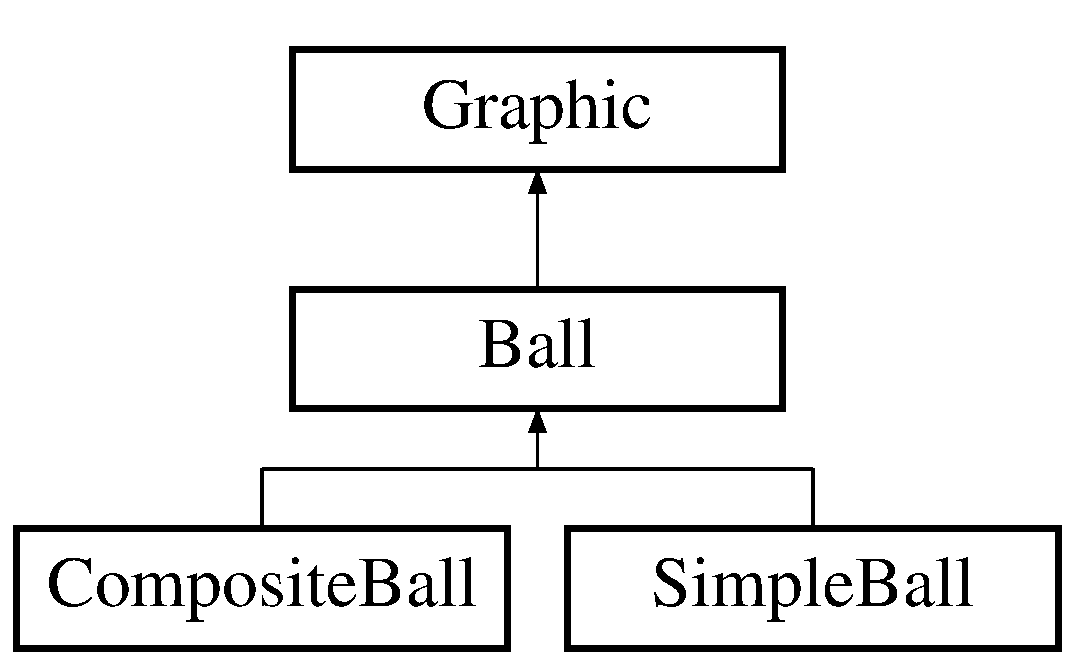
\includegraphics[height=3.000000cm]{class_ball}
\end{center}
\end{figure}
\subsection*{Public Member Functions}
\begin{DoxyCompactItemize}
\item 
\mbox{\hyperlink{class_ball_a52038e026ee4d3c960ec10e84465bfe2}{Ball}} (float radius=0, float mass=0, const Q\+Vector2D \&pos=N\+U\+L\+L\+\_\+2D, const Q\+Vector2D \&vel=N\+U\+L\+L\+\_\+2D, bool contained=false, bool is\+Remove=false)
\begin{DoxyCompactList}\small\item\em Constructor for ball. \end{DoxyCompactList}\item 
virtual void \mbox{\hyperlink{class_ball_a86aa99bb9b244c4ec9193f8ac09c6e8e}{change\+Pfor\+Contained}} (const Q\+Vector2D \&delta)=0
\begin{DoxyCompactList}\small\item\em change the position for the contained ball inside this ball, it is virtual and need to be overridden \end{DoxyCompactList}\item 
virtual float \mbox{\hyperlink{class_ball_ab755ce741a2f0b652f499d183376be04}{get\+Mass}} () const =0
\begin{DoxyCompactList}\small\item\em get the mass of the ball, virtual and need to be overridden \end{DoxyCompactList}\item 
virtual double \mbox{\hyperlink{class_ball_ab659c8dceb67abdd09423814d4fc879e}{get\+Strength}} () const =0
\begin{DoxyCompactList}\small\item\em get the stregnth of the ball, virtual and need to be overridden \end{DoxyCompactList}\item 
virtual int \mbox{\hyperlink{class_ball_a13794c8d0e0863301a5f321a617542f6}{get\+Contained\+Ball\+Number}} () const =0
\begin{DoxyCompactList}\small\item\em get the number of contained balls inside this ball, is virtual and need to be overridden \end{DoxyCompactList}\item 
virtual void \mbox{\hyperlink{class_ball_a43cfbf4dca89a94048b4d45b2eaf62e9}{change\+Vfor\+Contained}} (const Q\+Vector2D \&Parent\+Velocity, float energy\+Per\+Ball, const Q\+Vector2D \&point\+Of\+Collision) const =0
\begin{DoxyCompactList}\small\item\em change the velocity for contained balls inside this ball, is virtual and need to be overridden \end{DoxyCompactList}\item 
virtual void \mbox{\hyperlink{class_ball_a7d3b8c70ee8c61db73692a4d44bbf933}{move\+Out}} (std\+::vector$<$ unique\+\_\+ptr$<$ \mbox{\hyperlink{class_ball}{Ball}} $>$$>$ \&balls\+On\+Table)=0
\begin{DoxyCompactList}\small\item\em move the contained balls out into the input vector parameter, is virtual and need to be overridden \end{DoxyCompactList}\item 
virtual std\+::string \mbox{\hyperlink{class_ball_a248c8a5fc9b8770840f275ea7057b012}{get\+Colour}} () const =0
\begin{DoxyCompactList}\small\item\em get the colour of the ball, is virtual and need to be overridden \end{DoxyCompactList}\end{DoxyCompactItemize}
\subsection*{Public Attributes}
\begin{DoxyCompactItemize}
\item 
\mbox{\Hypertarget{class_ball_af9ccb63ad19e4073c1de2aadbcaaf542}\label{class_ball_af9ccb63ad19e4073c1de2aadbcaaf542}} 
bool {\bfseries is\+Contained}
\item 
\mbox{\Hypertarget{class_ball_a86bfb032007c736e06c2295a8070d620}\label{class_ball_a86bfb032007c736e06c2295a8070d620}} 
float {\bfseries radius}
\item 
\mbox{\Hypertarget{class_ball_a7d4dece3bb0e321f1739917ce8ff6297}\label{class_ball_a7d4dece3bb0e321f1739917ce8ff6297}} 
float {\bfseries mass}
\item 
\mbox{\Hypertarget{class_ball_af732a08aa15b235e44d30ca7a258f2be}\label{class_ball_af732a08aa15b235e44d30ca7a258f2be}} 
Q\+Vector2D {\bfseries position}
\item 
\mbox{\Hypertarget{class_ball_ad97aed858907a22482f53e5b623eaf6a}\label{class_ball_ad97aed858907a22482f53e5b623eaf6a}} 
Q\+Vector2D {\bfseries velocity}
\item 
\mbox{\Hypertarget{class_ball_ad50c5d8887de16a94113760871279743}\label{class_ball_ad50c5d8887de16a94113760871279743}} 
bool {\bfseries is\+Remove}
\end{DoxyCompactItemize}


\subsection{Detailed Description}
The \mbox{\hyperlink{class_ball}{Ball}} class is not responsible for physics calculation it exposes public radius position, velocity and mass fields so the responsible class can access them directly. You can pretend it\textquotesingle{}s a struct if you like. 

\subsection{Constructor \& Destructor Documentation}
\mbox{\Hypertarget{class_ball_a52038e026ee4d3c960ec10e84465bfe2}\label{class_ball_a52038e026ee4d3c960ec10e84465bfe2}} 
\index{Ball@{Ball}!Ball@{Ball}}
\index{Ball@{Ball}!Ball@{Ball}}
\subsubsection{\texorpdfstring{Ball()}{Ball()}}
{\footnotesize\ttfamily Ball\+::\+Ball (\begin{DoxyParamCaption}\item[{float}]{radius = {\ttfamily 0},  }\item[{float}]{mass = {\ttfamily 0},  }\item[{const Q\+Vector2D \&}]{pos = {\ttfamily NULL\+\_\+2D},  }\item[{const Q\+Vector2D \&}]{vel = {\ttfamily NULL\+\_\+2D},  }\item[{bool}]{contained = {\ttfamily false},  }\item[{bool}]{is\+Remove = {\ttfamily false} }\end{DoxyParamCaption})\hspace{0.3cm}{\ttfamily [inline]}}



Constructor for ball. 


\begin{DoxyParams}{Parameters}
{\em radius} & used for collision detection \\
\hline
{\em mass} & used for physics \\
\hline
{\em pos} & initial poisiton for the ball \\
\hline
{\em vel} & inital velocity for the ball \\
\hline
\end{DoxyParams}


\subsection{Member Function Documentation}
\mbox{\Hypertarget{class_ball_a86aa99bb9b244c4ec9193f8ac09c6e8e}\label{class_ball_a86aa99bb9b244c4ec9193f8ac09c6e8e}} 
\index{Ball@{Ball}!change\+Pfor\+Contained@{change\+Pfor\+Contained}}
\index{change\+Pfor\+Contained@{change\+Pfor\+Contained}!Ball@{Ball}}
\subsubsection{\texorpdfstring{change\+Pfor\+Contained()}{changePforContained()}}
{\footnotesize\ttfamily virtual void Ball\+::change\+Pfor\+Contained (\begin{DoxyParamCaption}\item[{const Q\+Vector2D \&}]{delta }\end{DoxyParamCaption})\hspace{0.3cm}{\ttfamily [pure virtual]}}



change the position for the contained ball inside this ball, it is virtual and need to be overridden 


\begin{DoxyParams}{Parameters}
{\em a} & Q\+Vector type carries the delta for position change \\
\hline
\end{DoxyParams}


Implemented in \mbox{\hyperlink{class_simple_ball_a22ec99de5d096383f869a919f9f9abd7}{Simple\+Ball}}, and \mbox{\hyperlink{class_composite_ball_a1e559c1b9d9b4905599c370c79990576}{Composite\+Ball}}.

\mbox{\Hypertarget{class_ball_a43cfbf4dca89a94048b4d45b2eaf62e9}\label{class_ball_a43cfbf4dca89a94048b4d45b2eaf62e9}} 
\index{Ball@{Ball}!change\+Vfor\+Contained@{change\+Vfor\+Contained}}
\index{change\+Vfor\+Contained@{change\+Vfor\+Contained}!Ball@{Ball}}
\subsubsection{\texorpdfstring{change\+Vfor\+Contained()}{changeVforContained()}}
{\footnotesize\ttfamily virtual void Ball\+::change\+Vfor\+Contained (\begin{DoxyParamCaption}\item[{const Q\+Vector2D \&}]{Parent\+Velocity,  }\item[{float}]{energy\+Per\+Ball,  }\item[{const Q\+Vector2D \&}]{point\+Of\+Collision }\end{DoxyParamCaption}) const\hspace{0.3cm}{\ttfamily [pure virtual]}}



change the velocity for contained balls inside this ball, is virtual and need to be overridden 


\begin{DoxyParams}{Parameters}
{\em a} & Q\+Vector2D of parent\textquotesingle{}s velocity \\
\hline
{\em a} & float of each ball\textquotesingle{}s energy \\
\hline
{\em a} & Q\+Vector2D of the collision\textquotesingle{}s point \\
\hline
\end{DoxyParams}


Implemented in \mbox{\hyperlink{class_simple_ball_a5e100bd3bc3b700d3ce1c5028d95ac31}{Simple\+Ball}}, and \mbox{\hyperlink{class_composite_ball_a9aa11bc758f517c35de751ae8ce27966}{Composite\+Ball}}.

\mbox{\Hypertarget{class_ball_a248c8a5fc9b8770840f275ea7057b012}\label{class_ball_a248c8a5fc9b8770840f275ea7057b012}} 
\index{Ball@{Ball}!get\+Colour@{get\+Colour}}
\index{get\+Colour@{get\+Colour}!Ball@{Ball}}
\subsubsection{\texorpdfstring{get\+Colour()}{getColour()}}
{\footnotesize\ttfamily virtual std\+::string Ball\+::get\+Colour (\begin{DoxyParamCaption}{ }\end{DoxyParamCaption}) const\hspace{0.3cm}{\ttfamily [pure virtual]}}



get the colour of the ball, is virtual and need to be overridden 

\begin{DoxyReturn}{Returns}
a string of the name of this colour 
\end{DoxyReturn}


Implemented in \mbox{\hyperlink{class_simple_ball_aad4437558814bc8c6f276d5e09507eb4}{Simple\+Ball}}, and \mbox{\hyperlink{class_composite_ball_aed883fc6572063ba2e3173e4a78ed6bf}{Composite\+Ball}}.

\mbox{\Hypertarget{class_ball_a13794c8d0e0863301a5f321a617542f6}\label{class_ball_a13794c8d0e0863301a5f321a617542f6}} 
\index{Ball@{Ball}!get\+Contained\+Ball\+Number@{get\+Contained\+Ball\+Number}}
\index{get\+Contained\+Ball\+Number@{get\+Contained\+Ball\+Number}!Ball@{Ball}}
\subsubsection{\texorpdfstring{get\+Contained\+Ball\+Number()}{getContainedBallNumber()}}
{\footnotesize\ttfamily virtual int Ball\+::get\+Contained\+Ball\+Number (\begin{DoxyParamCaption}{ }\end{DoxyParamCaption}) const\hspace{0.3cm}{\ttfamily [pure virtual]}}



get the number of contained balls inside this ball, is virtual and need to be overridden 

\begin{DoxyReturn}{Returns}
an interger of contained balls\textquotesingle{} number 
\end{DoxyReturn}


Implemented in \mbox{\hyperlink{class_simple_ball_ac9c7e389cf03bfb2f3e71d66bf6608cd}{Simple\+Ball}}, and \mbox{\hyperlink{class_composite_ball_a8120a00750a9bb77fd6e41f98de119b3}{Composite\+Ball}}.

\mbox{\Hypertarget{class_ball_ab755ce741a2f0b652f499d183376be04}\label{class_ball_ab755ce741a2f0b652f499d183376be04}} 
\index{Ball@{Ball}!get\+Mass@{get\+Mass}}
\index{get\+Mass@{get\+Mass}!Ball@{Ball}}
\subsubsection{\texorpdfstring{get\+Mass()}{getMass()}}
{\footnotesize\ttfamily virtual float Ball\+::get\+Mass (\begin{DoxyParamCaption}{ }\end{DoxyParamCaption}) const\hspace{0.3cm}{\ttfamily [pure virtual]}}



get the mass of the ball, virtual and need to be overridden 

\begin{DoxyReturn}{Returns}
a float type of mass 
\end{DoxyReturn}


Implemented in \mbox{\hyperlink{class_simple_ball_a0cb0b931a2e3fa9f2ffba6fd354985ea}{Simple\+Ball}}, and \mbox{\hyperlink{class_composite_ball_afa621612641fecb3af81390bfbe7d941}{Composite\+Ball}}.

\mbox{\Hypertarget{class_ball_ab659c8dceb67abdd09423814d4fc879e}\label{class_ball_ab659c8dceb67abdd09423814d4fc879e}} 
\index{Ball@{Ball}!get\+Strength@{get\+Strength}}
\index{get\+Strength@{get\+Strength}!Ball@{Ball}}
\subsubsection{\texorpdfstring{get\+Strength()}{getStrength()}}
{\footnotesize\ttfamily virtual double Ball\+::get\+Strength (\begin{DoxyParamCaption}{ }\end{DoxyParamCaption}) const\hspace{0.3cm}{\ttfamily [pure virtual]}}



get the stregnth of the ball, virtual and need to be overridden 

\begin{DoxyReturn}{Returns}
a double type of strength 
\end{DoxyReturn}


Implemented in \mbox{\hyperlink{class_simple_ball_a3a4c5bc776e3788112f02320432ba8cc}{Simple\+Ball}}, and \mbox{\hyperlink{class_composite_ball_a1585c03baf89ce19c58806dfa6eac131}{Composite\+Ball}}.

\mbox{\Hypertarget{class_ball_a7d3b8c70ee8c61db73692a4d44bbf933}\label{class_ball_a7d3b8c70ee8c61db73692a4d44bbf933}} 
\index{Ball@{Ball}!move\+Out@{move\+Out}}
\index{move\+Out@{move\+Out}!Ball@{Ball}}
\subsubsection{\texorpdfstring{move\+Out()}{moveOut()}}
{\footnotesize\ttfamily virtual void Ball\+::move\+Out (\begin{DoxyParamCaption}\item[{std\+::vector$<$ unique\+\_\+ptr$<$ \mbox{\hyperlink{class_ball}{Ball}} $>$$>$ \&}]{balls\+On\+Table }\end{DoxyParamCaption})\hspace{0.3cm}{\ttfamily [pure virtual]}}



move the contained balls out into the input vector parameter, is virtual and need to be overridden 


\begin{DoxyParams}{Parameters}
{\em a} & vector for balls on the table currently \\
\hline
\end{DoxyParams}


Implemented in \mbox{\hyperlink{class_simple_ball_a1af03353f6c3414e6ce7c12a9b338e72}{Simple\+Ball}}, and \mbox{\hyperlink{class_composite_ball_a2bf10829db0790d8a42529fafaf8c7b4}{Composite\+Ball}}.



The documentation for this class was generated from the following file\+:\begin{DoxyCompactItemize}
\item 
ball.\+h\end{DoxyCompactItemize}

\hypertarget{class_composite_ball}{}\section{Composite\+Ball Class Reference}
\label{class_composite_ball}\index{Composite\+Ball@{Composite\+Ball}}
Inheritance diagram for Composite\+Ball\+:\begin{figure}[H]
\begin{center}
\leavevmode
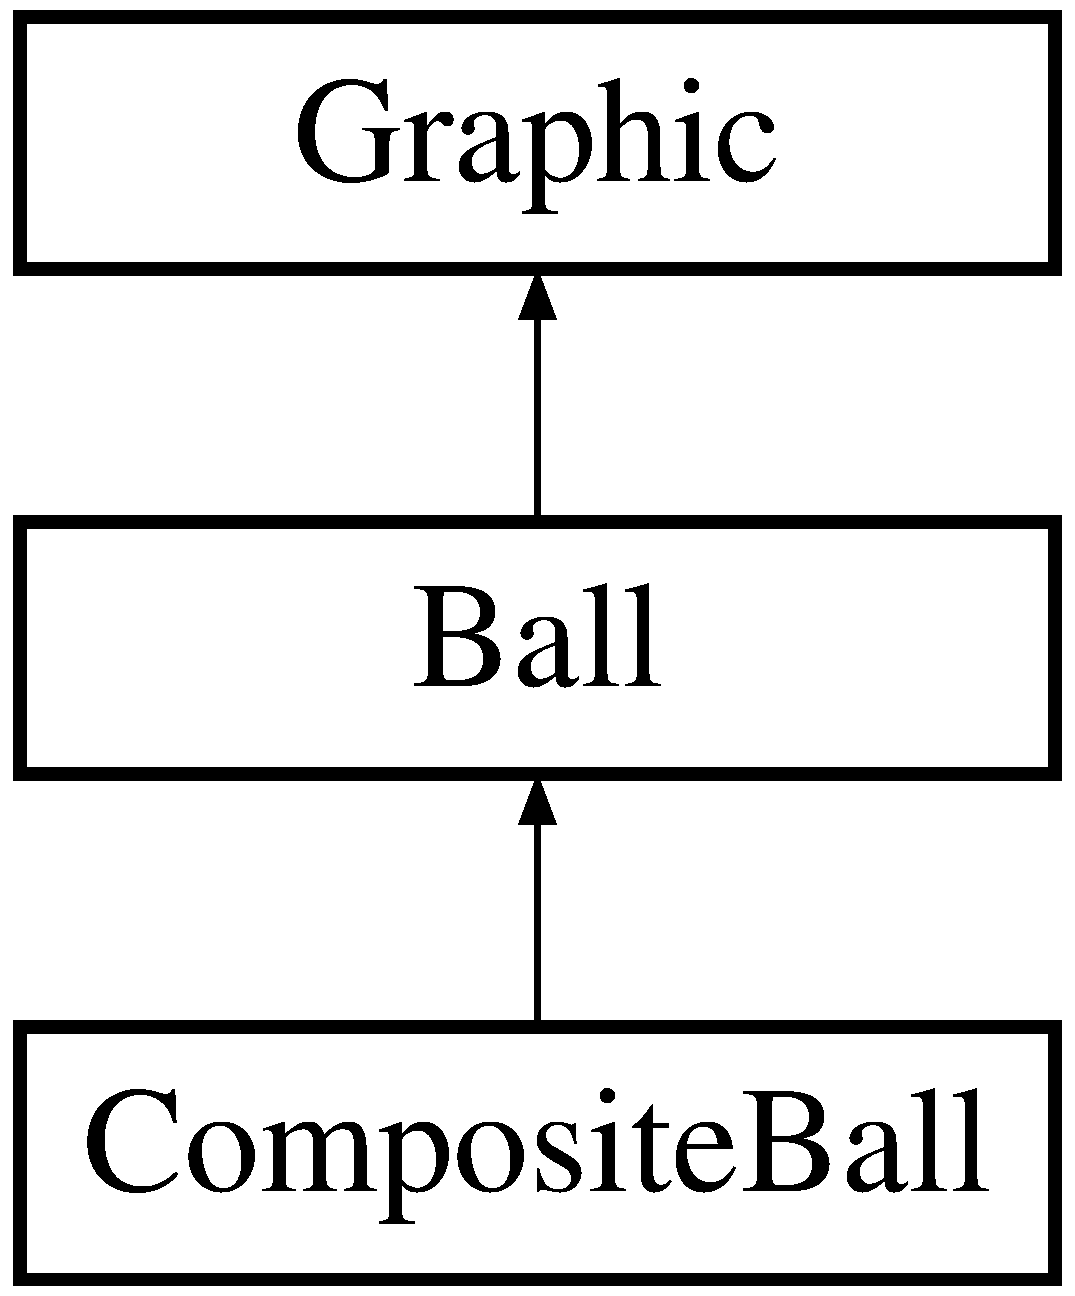
\includegraphics[height=3.000000cm]{class_composite_ball}
\end{center}
\end{figure}
\subsection*{Public Member Functions}
\begin{DoxyCompactItemize}
\item 
\mbox{\hyperlink{class_composite_ball_a5d9c99050f3844f59918fca2a1540cb4}{Composite\+Ball}} (float radius, float mass, const Q\+Vector2D \&pos, const Q\+Vector2D \&vel, const Q\+Color \&color, double strength, vector$<$ unique\+\_\+ptr$<$ \mbox{\hyperlink{class_ball}{Ball}} $>$$>$ \&balls, bool is\+Contained)
\begin{DoxyCompactList}\small\item\em constructor for composite ball \end{DoxyCompactList}\item 
void \mbox{\hyperlink{class_composite_ball_a976f7cc1cec45385c0a0f81cd69c2352}{draw}} (Q\+Painter \&painter) const override
\begin{DoxyCompactList}\small\item\em override the draw method to draw composite ball \end{DoxyCompactList}\item 
void \mbox{\hyperlink{class_composite_ball_a1e559c1b9d9b4905599c370c79990576}{change\+Pfor\+Contained}} (const Q\+Vector2D \&delta) override
\begin{DoxyCompactList}\small\item\em change the position for contained balls inside this ball \end{DoxyCompactList}\item 
float \mbox{\hyperlink{class_composite_ball_afa621612641fecb3af81390bfbe7d941}{get\+Mass}} () const override
\begin{DoxyCompactList}\small\item\em get the mass for this ball \end{DoxyCompactList}\item 
double \mbox{\hyperlink{class_composite_ball_a1585c03baf89ce19c58806dfa6eac131}{get\+Strength}} () const override
\begin{DoxyCompactList}\small\item\em get the strength of the ball \end{DoxyCompactList}\item 
int \mbox{\hyperlink{class_composite_ball_a8120a00750a9bb77fd6e41f98de119b3}{get\+Contained\+Ball\+Number}} () const override
\begin{DoxyCompactList}\small\item\em get the contained ball\textquotesingle{}s number \end{DoxyCompactList}\item 
void \mbox{\hyperlink{class_composite_ball_a9aa11bc758f517c35de751ae8ce27966}{change\+Vfor\+Contained}} (const Q\+Vector2D \&Parent\+Velocity, float energy\+Per\+Ball, const Q\+Vector2D \&point\+Of\+Collision) const override
\begin{DoxyCompactList}\small\item\em change the velocity for contained balls inside this ball \end{DoxyCompactList}\item 
void \mbox{\hyperlink{class_composite_ball_a2bf10829db0790d8a42529fafaf8c7b4}{move\+Out}} (std\+::vector$<$ unique\+\_\+ptr$<$ \mbox{\hyperlink{class_ball}{Ball}} $>$$>$ \&balls\+On\+Table) override
\begin{DoxyCompactList}\small\item\em move the contained balls out into the given vector \end{DoxyCompactList}\item 
std\+::string \mbox{\hyperlink{class_composite_ball_aed883fc6572063ba2e3173e4a78ed6bf}{get\+Colour}} () const override
\begin{DoxyCompactList}\small\item\em get the colour of this ball \end{DoxyCompactList}\end{DoxyCompactItemize}
\subsection*{Additional Inherited Members}


\subsection{Constructor \& Destructor Documentation}
\mbox{\Hypertarget{class_composite_ball_a5d9c99050f3844f59918fca2a1540cb4}\label{class_composite_ball_a5d9c99050f3844f59918fca2a1540cb4}} 
\index{Composite\+Ball@{Composite\+Ball}!Composite\+Ball@{Composite\+Ball}}
\index{Composite\+Ball@{Composite\+Ball}!Composite\+Ball@{Composite\+Ball}}
\subsubsection{\texorpdfstring{Composite\+Ball()}{CompositeBall()}}
{\footnotesize\ttfamily Composite\+Ball\+::\+Composite\+Ball (\begin{DoxyParamCaption}\item[{float}]{radius,  }\item[{float}]{mass,  }\item[{const Q\+Vector2D \&}]{pos,  }\item[{const Q\+Vector2D \&}]{vel,  }\item[{const Q\+Color \&}]{color,  }\item[{double}]{strength,  }\item[{vector$<$ unique\+\_\+ptr$<$ \mbox{\hyperlink{class_ball}{Ball}} $>$$>$ \&}]{balls,  }\item[{bool}]{is\+Contained }\end{DoxyParamCaption})}



constructor for composite ball 


\begin{DoxyParams}{Parameters}
{\em radius} & for the ball \\
\hline
{\em mass} & for the ball \\
\hline
{\em Q\+Vector2D} & position for the ball \\
\hline
{\em Q\+Vector2D} & velocity for the ball \\
\hline
{\em colour} & for the ball \\
\hline
{\em strength} & for the ball \\
\hline
\end{DoxyParams}


\subsection{Member Function Documentation}
\mbox{\Hypertarget{class_composite_ball_a1e559c1b9d9b4905599c370c79990576}\label{class_composite_ball_a1e559c1b9d9b4905599c370c79990576}} 
\index{Composite\+Ball@{Composite\+Ball}!change\+Pfor\+Contained@{change\+Pfor\+Contained}}
\index{change\+Pfor\+Contained@{change\+Pfor\+Contained}!Composite\+Ball@{Composite\+Ball}}
\subsubsection{\texorpdfstring{change\+Pfor\+Contained()}{changePforContained()}}
{\footnotesize\ttfamily void Composite\+Ball\+::change\+Pfor\+Contained (\begin{DoxyParamCaption}\item[{const Q\+Vector2D \&}]{delta }\end{DoxyParamCaption})\hspace{0.3cm}{\ttfamily [override]}, {\ttfamily [virtual]}}



change the position for contained balls inside this ball 


\begin{DoxyParams}{Parameters}
{\em delta} & position for changing \\
\hline
\end{DoxyParams}


Implements \mbox{\hyperlink{class_ball_a86aa99bb9b244c4ec9193f8ac09c6e8e}{Ball}}.

\mbox{\Hypertarget{class_composite_ball_a9aa11bc758f517c35de751ae8ce27966}\label{class_composite_ball_a9aa11bc758f517c35de751ae8ce27966}} 
\index{Composite\+Ball@{Composite\+Ball}!change\+Vfor\+Contained@{change\+Vfor\+Contained}}
\index{change\+Vfor\+Contained@{change\+Vfor\+Contained}!Composite\+Ball@{Composite\+Ball}}
\subsubsection{\texorpdfstring{change\+Vfor\+Contained()}{changeVforContained()}}
{\footnotesize\ttfamily void Composite\+Ball\+::change\+Vfor\+Contained (\begin{DoxyParamCaption}\item[{const Q\+Vector2D \&}]{Parent\+Velocity,  }\item[{float}]{energy\+Per\+Ball,  }\item[{const Q\+Vector2D \&}]{point\+Of\+Collision }\end{DoxyParamCaption}) const\hspace{0.3cm}{\ttfamily [override]}, {\ttfamily [virtual]}}



change the velocity for contained balls inside this ball 


\begin{DoxyParams}{Parameters}
{\em parent\textquotesingle{}s} & velocity \\
\hline
{\em after} & collision gained energy \\
\hline
{\em the} & point of collision \\
\hline
\end{DoxyParams}


Implements \mbox{\hyperlink{class_ball_a43cfbf4dca89a94048b4d45b2eaf62e9}{Ball}}.

\mbox{\Hypertarget{class_composite_ball_a976f7cc1cec45385c0a0f81cd69c2352}\label{class_composite_ball_a976f7cc1cec45385c0a0f81cd69c2352}} 
\index{Composite\+Ball@{Composite\+Ball}!draw@{draw}}
\index{draw@{draw}!Composite\+Ball@{Composite\+Ball}}
\subsubsection{\texorpdfstring{draw()}{draw()}}
{\footnotesize\ttfamily void Composite\+Ball\+::draw (\begin{DoxyParamCaption}\item[{Q\+Painter \&}]{painter }\end{DoxyParamCaption}) const\hspace{0.3cm}{\ttfamily [override]}, {\ttfamily [virtual]}}



override the draw method to draw composite ball 


\begin{DoxyParams}{Parameters}
{\em painter} & for drawing \\
\hline
\end{DoxyParams}


Implements \mbox{\hyperlink{class_graphic_aed0af75ae3756baeb3fe663ae5f36f29}{Graphic}}.

\mbox{\Hypertarget{class_composite_ball_aed883fc6572063ba2e3173e4a78ed6bf}\label{class_composite_ball_aed883fc6572063ba2e3173e4a78ed6bf}} 
\index{Composite\+Ball@{Composite\+Ball}!get\+Colour@{get\+Colour}}
\index{get\+Colour@{get\+Colour}!Composite\+Ball@{Composite\+Ball}}
\subsubsection{\texorpdfstring{get\+Colour()}{getColour()}}
{\footnotesize\ttfamily std\+::string Composite\+Ball\+::get\+Colour (\begin{DoxyParamCaption}{ }\end{DoxyParamCaption}) const\hspace{0.3cm}{\ttfamily [override]}, {\ttfamily [virtual]}}



get the colour of this ball 

\begin{DoxyReturn}{Returns}
return the string type of the colour name 
\end{DoxyReturn}


Implements \mbox{\hyperlink{class_ball_a248c8a5fc9b8770840f275ea7057b012}{Ball}}.

\mbox{\Hypertarget{class_composite_ball_a8120a00750a9bb77fd6e41f98de119b3}\label{class_composite_ball_a8120a00750a9bb77fd6e41f98de119b3}} 
\index{Composite\+Ball@{Composite\+Ball}!get\+Contained\+Ball\+Number@{get\+Contained\+Ball\+Number}}
\index{get\+Contained\+Ball\+Number@{get\+Contained\+Ball\+Number}!Composite\+Ball@{Composite\+Ball}}
\subsubsection{\texorpdfstring{get\+Contained\+Ball\+Number()}{getContainedBallNumber()}}
{\footnotesize\ttfamily int Composite\+Ball\+::get\+Contained\+Ball\+Number (\begin{DoxyParamCaption}{ }\end{DoxyParamCaption}) const\hspace{0.3cm}{\ttfamily [override]}, {\ttfamily [virtual]}}



get the contained ball\textquotesingle{}s number 

\begin{DoxyReturn}{Returns}
an interger of number 
\end{DoxyReturn}


Implements \mbox{\hyperlink{class_ball_a13794c8d0e0863301a5f321a617542f6}{Ball}}.

\mbox{\Hypertarget{class_composite_ball_afa621612641fecb3af81390bfbe7d941}\label{class_composite_ball_afa621612641fecb3af81390bfbe7d941}} 
\index{Composite\+Ball@{Composite\+Ball}!get\+Mass@{get\+Mass}}
\index{get\+Mass@{get\+Mass}!Composite\+Ball@{Composite\+Ball}}
\subsubsection{\texorpdfstring{get\+Mass()}{getMass()}}
{\footnotesize\ttfamily float Composite\+Ball\+::get\+Mass (\begin{DoxyParamCaption}{ }\end{DoxyParamCaption}) const\hspace{0.3cm}{\ttfamily [override]}, {\ttfamily [virtual]}}



get the mass for this ball 

\begin{DoxyReturn}{Returns}
a float type of mass 
\end{DoxyReturn}


Implements \mbox{\hyperlink{class_ball_ab755ce741a2f0b652f499d183376be04}{Ball}}.

\mbox{\Hypertarget{class_composite_ball_a1585c03baf89ce19c58806dfa6eac131}\label{class_composite_ball_a1585c03baf89ce19c58806dfa6eac131}} 
\index{Composite\+Ball@{Composite\+Ball}!get\+Strength@{get\+Strength}}
\index{get\+Strength@{get\+Strength}!Composite\+Ball@{Composite\+Ball}}
\subsubsection{\texorpdfstring{get\+Strength()}{getStrength()}}
{\footnotesize\ttfamily double Composite\+Ball\+::get\+Strength (\begin{DoxyParamCaption}{ }\end{DoxyParamCaption}) const\hspace{0.3cm}{\ttfamily [override]}, {\ttfamily [virtual]}}



get the strength of the ball 

\begin{DoxyReturn}{Returns}
a double type of strength 
\end{DoxyReturn}


Implements \mbox{\hyperlink{class_ball_ab659c8dceb67abdd09423814d4fc879e}{Ball}}.

\mbox{\Hypertarget{class_composite_ball_a2bf10829db0790d8a42529fafaf8c7b4}\label{class_composite_ball_a2bf10829db0790d8a42529fafaf8c7b4}} 
\index{Composite\+Ball@{Composite\+Ball}!move\+Out@{move\+Out}}
\index{move\+Out@{move\+Out}!Composite\+Ball@{Composite\+Ball}}
\subsubsection{\texorpdfstring{move\+Out()}{moveOut()}}
{\footnotesize\ttfamily void Composite\+Ball\+::move\+Out (\begin{DoxyParamCaption}\item[{std\+::vector$<$ unique\+\_\+ptr$<$ \mbox{\hyperlink{class_ball}{Ball}} $>$$>$ \&}]{balls\+On\+Table }\end{DoxyParamCaption})\hspace{0.3cm}{\ttfamily [override]}, {\ttfamily [virtual]}}



move the contained balls out into the given vector 


\begin{DoxyParams}{Parameters}
{\em given} & vector as destination for contained balls \\
\hline
\end{DoxyParams}


Implements \mbox{\hyperlink{class_ball_a7d3b8c70ee8c61db73692a4d44bbf933}{Ball}}.



The documentation for this class was generated from the following files\+:\begin{DoxyCompactItemize}
\item 
compositeball.\+h\item 
compositeball.\+cpp\end{DoxyCompactItemize}

\hypertarget{class_creator}{}\section{Creator Class Reference}
\label{class_creator}\index{Creator@{Creator}}
Inheritance diagram for Creator\+:\begin{figure}[H]
\begin{center}
\leavevmode
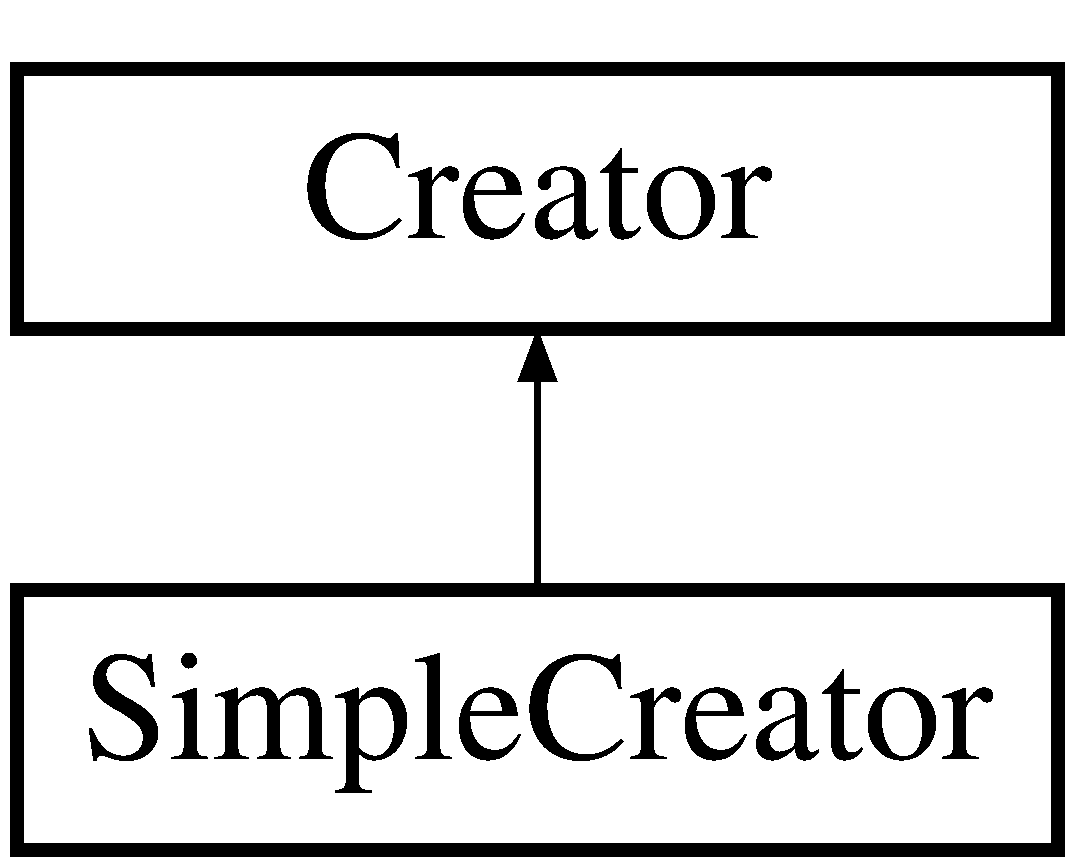
\includegraphics[height=2.000000cm]{class_creator}
\end{center}
\end{figure}
\subsection*{Public Member Functions}
\begin{DoxyCompactItemize}
\item 
unique\+\_\+ptr$<$ \mbox{\hyperlink{class_scene_manager}{Scene\+Manager}} $>$ \mbox{\hyperlink{class_creator_ae2ccbd8403068b381ad49e6c3b39891f}{make\+Scene}} (const Q\+Json\+Object \&spec)
\begin{DoxyCompactList}\small\item\em used for initialising a \mbox{\hyperlink{class_scene_manager}{Scene\+Manager}} from a J\+S\+ON configuration \end{DoxyCompactList}\end{DoxyCompactItemize}
\subsection*{Protected Member Functions}
\begin{DoxyCompactItemize}
\item 
virtual unique\+\_\+ptr$<$ \mbox{\hyperlink{class_table}{Table}} $>$ \mbox{\hyperlink{class_creator_a70c571c0b776a5f29494f660957e0710}{make\+Table}} (const Q\+Json\+Object \&spec, int f=1)=0
\begin{DoxyCompactList}\small\item\em makes a (concrete) \mbox{\hyperlink{class_table}{Table}} from J\+S\+ON config implemented by subclass \end{DoxyCompactList}\item 
virtual unique\+\_\+ptr$<$ \mbox{\hyperlink{class_ball}{Ball}} $>$ \mbox{\hyperlink{class_creator_aa3f6415656f52625d4f3051bfa70d4eb}{make\+Ball}} (const Q\+Json\+Object \&spec, int f=1)=0
\begin{DoxyCompactList}\small\item\em makes a (concrete) \mbox{\hyperlink{class_ball}{Ball}} from J\+S\+ON config implemented by subclass \end{DoxyCompactList}\end{DoxyCompactItemize}


\subsection{Member Function Documentation}
\mbox{\Hypertarget{class_creator_aa3f6415656f52625d4f3051bfa70d4eb}\label{class_creator_aa3f6415656f52625d4f3051bfa70d4eb}} 
\index{Creator@{Creator}!make\+Ball@{make\+Ball}}
\index{make\+Ball@{make\+Ball}!Creator@{Creator}}
\subsubsection{\texorpdfstring{make\+Ball()}{makeBall()}}
{\footnotesize\ttfamily virtual unique\+\_\+ptr$<$\mbox{\hyperlink{class_ball}{Ball}}$>$ Creator\+::make\+Ball (\begin{DoxyParamCaption}\item[{const Q\+Json\+Object \&}]{spec,  }\item[{int}]{f = {\ttfamily 1} }\end{DoxyParamCaption})\hspace{0.3cm}{\ttfamily [protected]}, {\ttfamily [pure virtual]}}



makes a (concrete) \mbox{\hyperlink{class_ball}{Ball}} from J\+S\+ON config implemented by subclass 


\begin{DoxyParams}{Parameters}
{\em spec} & a J\+S\+ON object detailing the properties of the ball\\
\hline
\end{DoxyParams}
\begin{DoxyReturn}{Returns}
a \mbox{\hyperlink{class_ball}{Ball}} with the specified property 
\end{DoxyReturn}


Implemented in \mbox{\hyperlink{class_simple_creator_a8e5fdfc8bcd5a661cdcfb49d33a51910}{Simple\+Creator}}.

\mbox{\Hypertarget{class_creator_ae2ccbd8403068b381ad49e6c3b39891f}\label{class_creator_ae2ccbd8403068b381ad49e6c3b39891f}} 
\index{Creator@{Creator}!make\+Scene@{make\+Scene}}
\index{make\+Scene@{make\+Scene}!Creator@{Creator}}
\subsubsection{\texorpdfstring{make\+Scene()}{makeScene()}}
{\footnotesize\ttfamily unique\+\_\+ptr$<$ \mbox{\hyperlink{class_scene_manager}{Scene\+Manager}} $>$ Creator\+::make\+Scene (\begin{DoxyParamCaption}\item[{const Q\+Json\+Object \&}]{spec }\end{DoxyParamCaption})}



used for initialising a \mbox{\hyperlink{class_scene_manager}{Scene\+Manager}} from a J\+S\+ON configuration 


\begin{DoxyParams}{Parameters}
{\em spec} & a J\+S\+ON object detailing the initial property of the scene including a table and balls\\
\hline
\end{DoxyParams}
\begin{DoxyReturn}{Returns}
a \mbox{\hyperlink{class_scene_manager}{Scene\+Manager}} with the specified properties 
\end{DoxyReturn}
\mbox{\Hypertarget{class_creator_a70c571c0b776a5f29494f660957e0710}\label{class_creator_a70c571c0b776a5f29494f660957e0710}} 
\index{Creator@{Creator}!make\+Table@{make\+Table}}
\index{make\+Table@{make\+Table}!Creator@{Creator}}
\subsubsection{\texorpdfstring{make\+Table()}{makeTable()}}
{\footnotesize\ttfamily virtual unique\+\_\+ptr$<$\mbox{\hyperlink{class_table}{Table}}$>$ Creator\+::make\+Table (\begin{DoxyParamCaption}\item[{const Q\+Json\+Object \&}]{spec,  }\item[{int}]{f = {\ttfamily 1} }\end{DoxyParamCaption})\hspace{0.3cm}{\ttfamily [protected]}, {\ttfamily [pure virtual]}}



makes a (concrete) \mbox{\hyperlink{class_table}{Table}} from J\+S\+ON config implemented by subclass 


\begin{DoxyParams}{Parameters}
{\em spec} & a J\+S\+ON object detailing the properties of the table\\
\hline
\end{DoxyParams}
\begin{DoxyReturn}{Returns}
a \mbox{\hyperlink{class_table}{Table}} with the specified property 
\end{DoxyReturn}


Implemented in \mbox{\hyperlink{class_simple_creator_af6556afca4e573deaaf624e8be14dfae}{Simple\+Creator}}.



The documentation for this class was generated from the following files\+:\begin{DoxyCompactItemize}
\item 
creator.\+h\item 
creator.\+cpp\end{DoxyCompactItemize}

\hypertarget{class_graphic}{}\section{Graphic Class Reference}
\label{class_graphic}\index{Graphic@{Graphic}}
Inheritance diagram for Graphic\+:\begin{figure}[H]
\begin{center}
\leavevmode
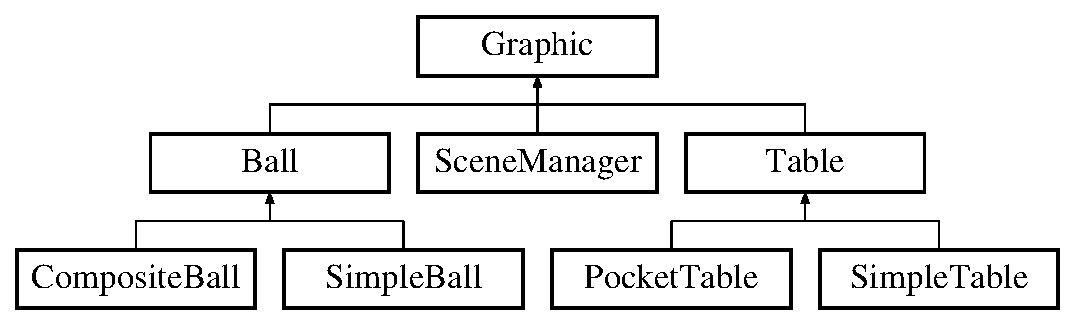
\includegraphics[height=3.000000cm]{class_graphic}
\end{center}
\end{figure}
\subsection*{Public Member Functions}
\begin{DoxyCompactItemize}
\item 
virtual void \mbox{\hyperlink{class_graphic_aed0af75ae3756baeb3fe663ae5f36f29}{draw}} (Q\+Painter \&painter) const =0
\begin{DoxyCompactList}\small\item\em an interface for rendering object on Qt \end{DoxyCompactList}\end{DoxyCompactItemize}


\subsection{Member Function Documentation}
\mbox{\Hypertarget{class_graphic_aed0af75ae3756baeb3fe663ae5f36f29}\label{class_graphic_aed0af75ae3756baeb3fe663ae5f36f29}} 
\index{Graphic@{Graphic}!draw@{draw}}
\index{draw@{draw}!Graphic@{Graphic}}
\subsubsection{\texorpdfstring{draw()}{draw()}}
{\footnotesize\ttfamily virtual void Graphic\+::draw (\begin{DoxyParamCaption}\item[{Q\+Painter \&}]{painter }\end{DoxyParamCaption}) const\hspace{0.3cm}{\ttfamily [pure virtual]}}



an interface for rendering object on Qt 


\begin{DoxyParams}{Parameters}
{\em painter} & for rendering the object \\
\hline
\end{DoxyParams}


Implemented in \mbox{\hyperlink{class_scene_manager_a1acae2e8e78a37c3cb17c5d90a5882ca}{Scene\+Manager}}, \mbox{\hyperlink{class_simple_ball_ad775dddec77276d6f92f8aea4b487df3}{Simple\+Ball}}, \mbox{\hyperlink{class_composite_ball_a976f7cc1cec45385c0a0f81cd69c2352}{Composite\+Ball}}, \mbox{\hyperlink{class_pocket_table_ab7c2954c1723c070836b453fe0a3bf67}{Pocket\+Table}}, and \mbox{\hyperlink{class_simple_table_aabb9fe0665f1145ba620c1f6ff9b5576}{Simple\+Table}}.



The documentation for this class was generated from the following file\+:\begin{DoxyCompactItemize}
\item 
graphic.\+h\end{DoxyCompactItemize}

\hypertarget{class_main_window}{}\section{Main\+Window Class Reference}
\label{class_main_window}\index{Main\+Window@{Main\+Window}}


The top level class for controlling the window.  




{\ttfamily \#include $<$mainwindow.\+h$>$}

Inheritance diagram for Main\+Window\+:\begin{figure}[H]
\begin{center}
\leavevmode
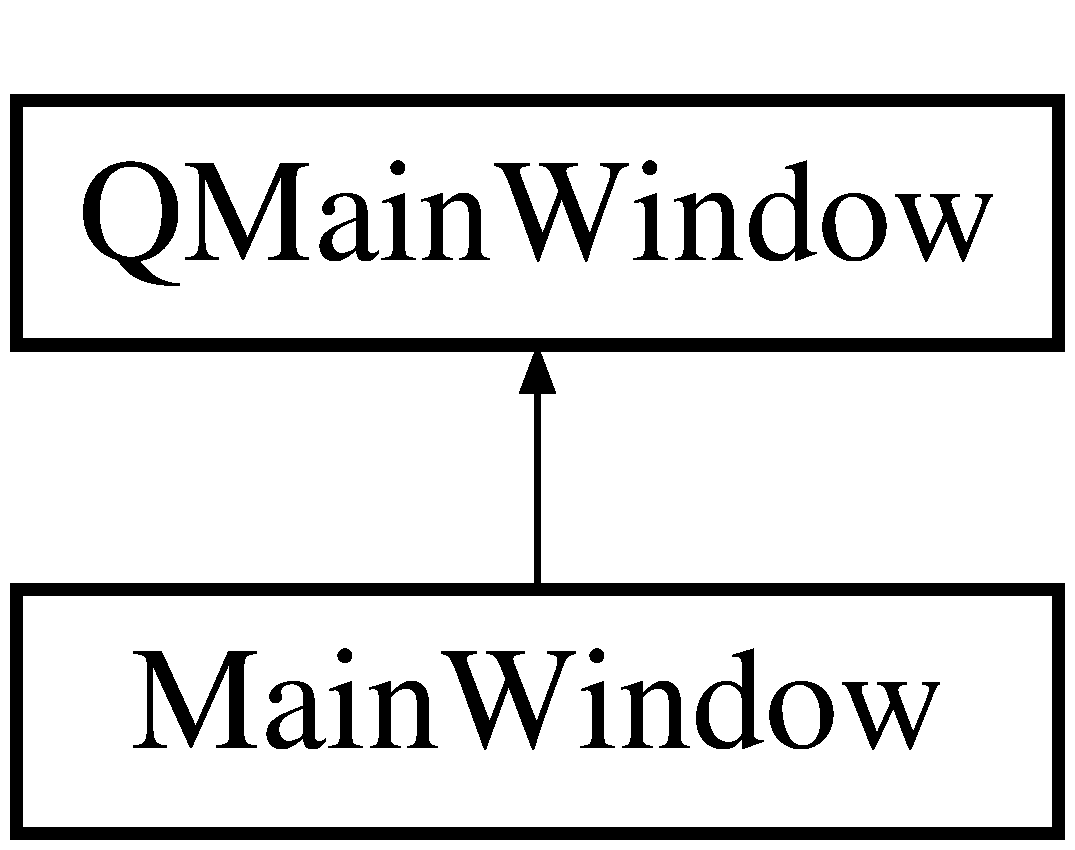
\includegraphics[height=2.000000cm]{class_main_window}
\end{center}
\end{figure}
\subsection*{Public Slots}
\begin{DoxyCompactItemize}
\item 
\mbox{\Hypertarget{class_main_window_a48965b8c40edf53d61e2d41977c1566d}\label{class_main_window_a48965b8c40edf53d61e2d41977c1566d}} 
void \mbox{\hyperlink{class_main_window_a48965b8c40edf53d61e2d41977c1566d}{tick}} ()
\begin{DoxyCompactList}\small\item\em move the scene by a small timestep \end{DoxyCompactList}\item 
\mbox{\Hypertarget{class_main_window_a4c2deac99b9b27dbb251d52380150515}\label{class_main_window_a4c2deac99b9b27dbb251d52380150515}} 
void \mbox{\hyperlink{class_main_window_a4c2deac99b9b27dbb251d52380150515}{next\+Frame}} ()
\begin{DoxyCompactList}\small\item\em draws the next frame \end{DoxyCompactList}\end{DoxyCompactItemize}
\subsection*{Public Member Functions}
\begin{DoxyCompactItemize}
\item 
\mbox{\hyperlink{class_main_window_af5ee499b2fb8e1ece871f21acc9dd332}{Main\+Window}} (unique\+\_\+ptr$<$ \mbox{\hyperlink{class_scene_manager}{Scene\+Manager}} $>$ scene, Q\+Widget $\ast$parent=0)
\begin{DoxyCompactList}\small\item\em Constructor. \end{DoxyCompactList}\end{DoxyCompactItemize}
\subsection*{Protected Member Functions}
\begin{DoxyCompactItemize}
\item 
void \mbox{\hyperlink{class_main_window_a1dff511c9697cbcb60150894f480b9c8}{mouse\+Press\+Event}} (Q\+Mouse\+Event $\ast$event) override
\begin{DoxyCompactList}\small\item\em the event for pressing mouse\+: record the cursor position \end{DoxyCompactList}\item 
void \mbox{\hyperlink{class_main_window_ad162aaba235ea093b59f6a9bf0fc4d01}{mouse\+Release\+Event}} (Q\+Mouse\+Event $\ast$event) override
\begin{DoxyCompactList}\small\item\em the event for releasing mouse\+: record the position \end{DoxyCompactList}\item 
void \mbox{\hyperlink{class_main_window_a9c8748d463f01ddae6abcd8f8163fcef}{mouse\+Move\+Event}} (Q\+Mouse\+Event $\ast$event) override
\begin{DoxyCompactList}\small\item\em the event for moving mouse\+: get current cursor position \end{DoxyCompactList}\item 
void \mbox{\hyperlink{class_main_window_abf05d580e91f725777cdb6a5eb0bf08c}{paint\+Event}} (Q\+Paint\+Event $\ast$event)
\begin{DoxyCompactList}\small\item\em draws objects on the window \end{DoxyCompactList}\end{DoxyCompactItemize}


\subsection{Detailed Description}
The top level class for controlling the window. 

\subsection{Constructor \& Destructor Documentation}
\mbox{\Hypertarget{class_main_window_af5ee499b2fb8e1ece871f21acc9dd332}\label{class_main_window_af5ee499b2fb8e1ece871f21acc9dd332}} 
\index{Main\+Window@{Main\+Window}!Main\+Window@{Main\+Window}}
\index{Main\+Window@{Main\+Window}!Main\+Window@{Main\+Window}}
\subsubsection{\texorpdfstring{Main\+Window()}{MainWindow()}}
{\footnotesize\ttfamily Main\+Window\+::\+Main\+Window (\begin{DoxyParamCaption}\item[{unique\+\_\+ptr$<$ \mbox{\hyperlink{class_scene_manager}{Scene\+Manager}} $>$}]{scene,  }\item[{Q\+Widget $\ast$}]{parent = {\ttfamily 0} }\end{DoxyParamCaption})}



Constructor. 


\begin{DoxyParams}{Parameters}
{\em scene} & a Scene for the program to render \\
\hline
{\em parent} & the parent Qt Object \\
\hline
\end{DoxyParams}


\subsection{Member Function Documentation}
\mbox{\Hypertarget{class_main_window_a9c8748d463f01ddae6abcd8f8163fcef}\label{class_main_window_a9c8748d463f01ddae6abcd8f8163fcef}} 
\index{Main\+Window@{Main\+Window}!mouse\+Move\+Event@{mouse\+Move\+Event}}
\index{mouse\+Move\+Event@{mouse\+Move\+Event}!Main\+Window@{Main\+Window}}
\subsubsection{\texorpdfstring{mouse\+Move\+Event()}{mouseMoveEvent()}}
{\footnotesize\ttfamily void Main\+Window\+::mouse\+Move\+Event (\begin{DoxyParamCaption}\item[{Q\+Mouse\+Event $\ast$}]{event }\end{DoxyParamCaption})\hspace{0.3cm}{\ttfamily [override]}, {\ttfamily [protected]}}



the event for moving mouse\+: get current cursor position 


\begin{DoxyParams}{Parameters}
{\em Q\+Mouse\+Event} & object \\
\hline
\end{DoxyParams}
\mbox{\Hypertarget{class_main_window_a1dff511c9697cbcb60150894f480b9c8}\label{class_main_window_a1dff511c9697cbcb60150894f480b9c8}} 
\index{Main\+Window@{Main\+Window}!mouse\+Press\+Event@{mouse\+Press\+Event}}
\index{mouse\+Press\+Event@{mouse\+Press\+Event}!Main\+Window@{Main\+Window}}
\subsubsection{\texorpdfstring{mouse\+Press\+Event()}{mousePressEvent()}}
{\footnotesize\ttfamily void Main\+Window\+::mouse\+Press\+Event (\begin{DoxyParamCaption}\item[{Q\+Mouse\+Event $\ast$}]{event }\end{DoxyParamCaption})\hspace{0.3cm}{\ttfamily [override]}, {\ttfamily [protected]}}



the event for pressing mouse\+: record the cursor position 


\begin{DoxyParams}{Parameters}
{\em Q\+Mouse\+Event} & object \\
\hline
\end{DoxyParams}
\mbox{\Hypertarget{class_main_window_ad162aaba235ea093b59f6a9bf0fc4d01}\label{class_main_window_ad162aaba235ea093b59f6a9bf0fc4d01}} 
\index{Main\+Window@{Main\+Window}!mouse\+Release\+Event@{mouse\+Release\+Event}}
\index{mouse\+Release\+Event@{mouse\+Release\+Event}!Main\+Window@{Main\+Window}}
\subsubsection{\texorpdfstring{mouse\+Release\+Event()}{mouseReleaseEvent()}}
{\footnotesize\ttfamily void Main\+Window\+::mouse\+Release\+Event (\begin{DoxyParamCaption}\item[{Q\+Mouse\+Event $\ast$}]{event }\end{DoxyParamCaption})\hspace{0.3cm}{\ttfamily [override]}, {\ttfamily [protected]}}



the event for releasing mouse\+: record the position 


\begin{DoxyParams}{Parameters}
{\em Q\+Mouse\+Event} & object \\
\hline
\end{DoxyParams}
\mbox{\Hypertarget{class_main_window_abf05d580e91f725777cdb6a5eb0bf08c}\label{class_main_window_abf05d580e91f725777cdb6a5eb0bf08c}} 
\index{Main\+Window@{Main\+Window}!paint\+Event@{paint\+Event}}
\index{paint\+Event@{paint\+Event}!Main\+Window@{Main\+Window}}
\subsubsection{\texorpdfstring{paint\+Event()}{paintEvent()}}
{\footnotesize\ttfamily void Main\+Window\+::paint\+Event (\begin{DoxyParamCaption}\item[{Q\+Paint\+Event $\ast$}]{event }\end{DoxyParamCaption})\hspace{0.3cm}{\ttfamily [protected]}}



draws objects on the window 


\begin{DoxyParams}{Parameters}
{\em event} & specifies regions to render \\
\hline
\end{DoxyParams}


The documentation for this class was generated from the following files\+:\begin{DoxyCompactItemize}
\item 
mainwindow.\+h\item 
mainwindow.\+cpp\end{DoxyCompactItemize}

\hypertarget{class_pocket}{}\section{Pocket Class Reference}
\label{class_pocket}\index{Pocket@{Pocket}}
\subsection*{Public Member Functions}
\begin{DoxyCompactItemize}
\item 
\mbox{\hyperlink{class_pocket_a8097676f321bbe9f8827b3e1bf970b85}{Pocket}} (const Q\+Vector2D \&pos=N\+U\+L\+L\+\_\+2D, float radius=15)
\begin{DoxyCompactList}\small\item\em constructor for pocket \end{DoxyCompactList}\end{DoxyCompactItemize}
\subsection*{Public Attributes}
\begin{DoxyCompactItemize}
\item 
\mbox{\Hypertarget{class_pocket_abed1a0b9e00fd3701a94ef36b87c9ba4}\label{class_pocket_abed1a0b9e00fd3701a94ef36b87c9ba4}} 
float {\bfseries radius}
\item 
\mbox{\Hypertarget{class_pocket_a68d67c1e98642a2e8f47192ded1abb97}\label{class_pocket_a68d67c1e98642a2e8f47192ded1abb97}} 
Q\+Vector2D {\bfseries position}
\end{DoxyCompactItemize}


\subsection{Constructor \& Destructor Documentation}
\mbox{\Hypertarget{class_pocket_a8097676f321bbe9f8827b3e1bf970b85}\label{class_pocket_a8097676f321bbe9f8827b3e1bf970b85}} 
\index{Pocket@{Pocket}!Pocket@{Pocket}}
\index{Pocket@{Pocket}!Pocket@{Pocket}}
\subsubsection{\texorpdfstring{Pocket()}{Pocket()}}
{\footnotesize\ttfamily Pocket\+::\+Pocket (\begin{DoxyParamCaption}\item[{const Q\+Vector2D \&}]{pos = {\ttfamily NULL\+\_\+2D},  }\item[{float}]{radius = {\ttfamily 15} }\end{DoxyParamCaption})}



constructor for pocket 


\begin{DoxyParams}{Parameters}
{\em position} & of the pocket \\
\hline
{\em redius} & of the pocket \\
\hline
\end{DoxyParams}


The documentation for this class was generated from the following files\+:\begin{DoxyCompactItemize}
\item 
pocket.\+h\item 
pocket.\+cpp\end{DoxyCompactItemize}

\hypertarget{class_pocket_table}{}\section{Pocket\+Table Class Reference}
\label{class_pocket_table}\index{Pocket\+Table@{Pocket\+Table}}
Inheritance diagram for Pocket\+Table\+:\begin{figure}[H]
\begin{center}
\leavevmode
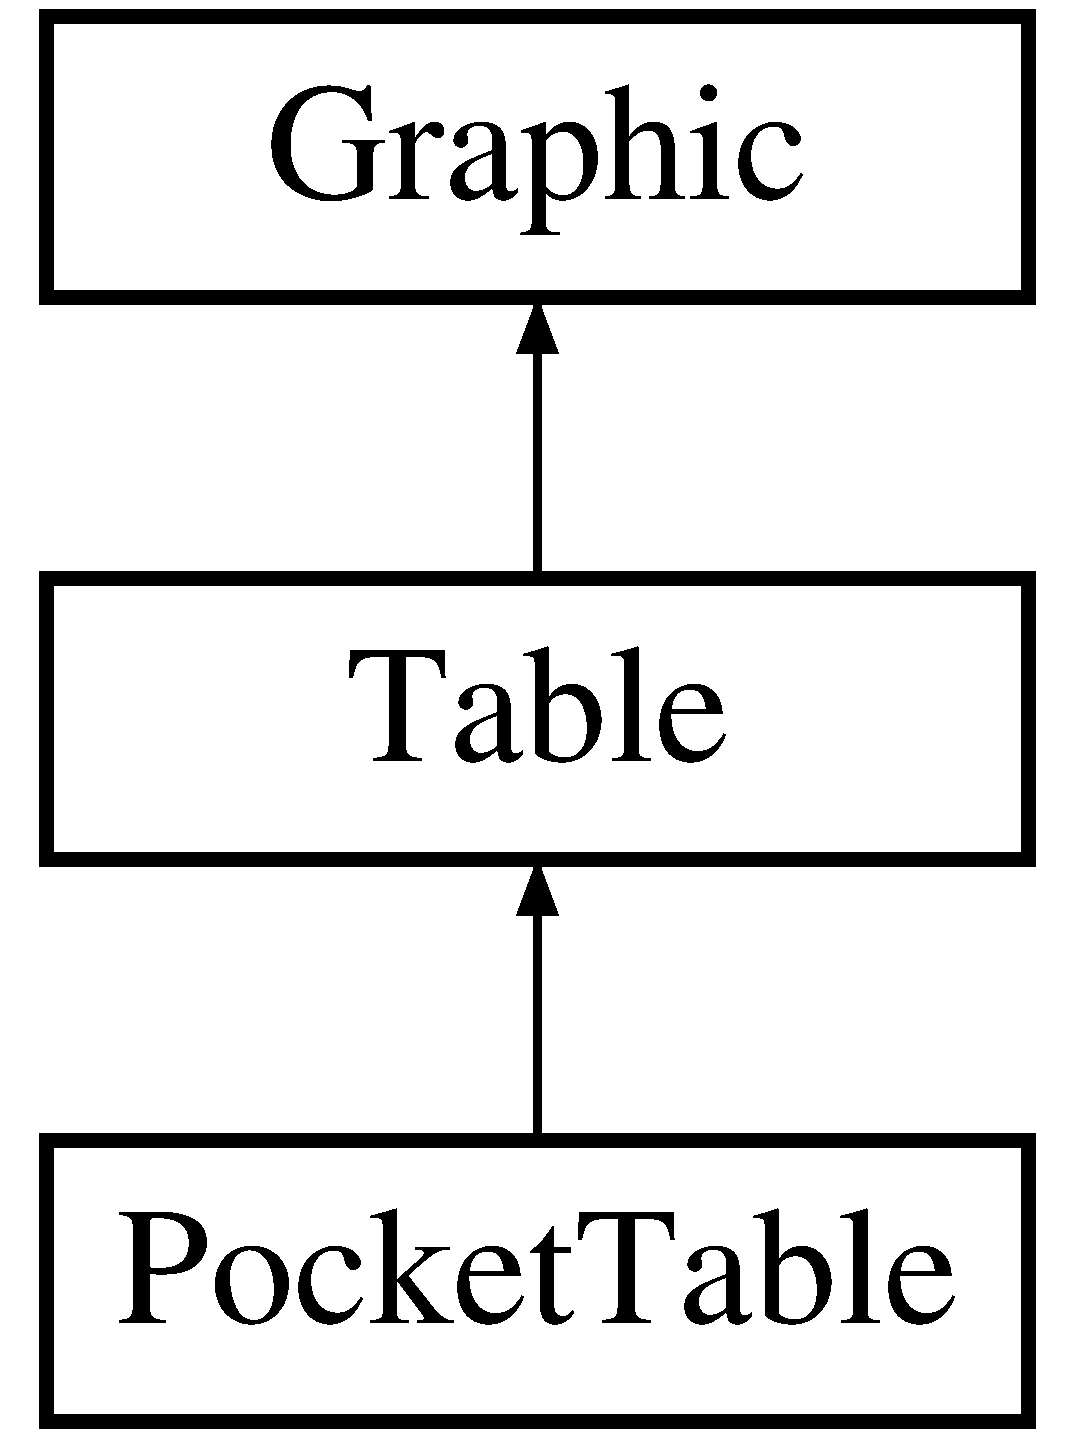
\includegraphics[height=3.000000cm]{class_pocket_table}
\end{center}
\end{figure}
\subsection*{Public Member Functions}
\begin{DoxyCompactItemize}
\item 
\mbox{\hyperlink{class_pocket_table_a774e36c15c5fda9070c8ed13abb49950}{Pocket\+Table}} (unique\+\_\+ptr$<$ \mbox{\hyperlink{class_simple_table}{Simple\+Table}} $>$ table, vector$<$ unique\+\_\+ptr$<$ \mbox{\hyperlink{class_pocket}{Pocket}} $>$$>$ \&pockets, const Q\+Size \&dim, float friction, vector$<$ unique\+\_\+ptr$<$ \mbox{\hyperlink{class_pocket}{Pocket}} $>$$>$ \&pockets1)
\begin{DoxyCompactList}\small\item\em constructor for table with pockets implemented by the decorator pattern \end{DoxyCompactList}\item 
void \mbox{\hyperlink{class_pocket_table_ab7c2954c1723c070836b453fe0a3bf67}{draw}} (Q\+Painter \&painter) const
\begin{DoxyCompactList}\small\item\em draw method for table with pocket \end{DoxyCompactList}\end{DoxyCompactItemize}
\subsection*{Public Attributes}
\begin{DoxyCompactItemize}
\item 
\mbox{\Hypertarget{class_pocket_table_a5b0f120d075425febbf04939198490dd}\label{class_pocket_table_a5b0f120d075425febbf04939198490dd}} 
vector$<$ unique\+\_\+ptr$<$ \mbox{\hyperlink{class_pocket}{Pocket}} $>$ $>$ {\bfseries pockets}
\end{DoxyCompactItemize}


\subsection{Constructor \& Destructor Documentation}
\mbox{\Hypertarget{class_pocket_table_a774e36c15c5fda9070c8ed13abb49950}\label{class_pocket_table_a774e36c15c5fda9070c8ed13abb49950}} 
\index{Pocket\+Table@{Pocket\+Table}!Pocket\+Table@{Pocket\+Table}}
\index{Pocket\+Table@{Pocket\+Table}!Pocket\+Table@{Pocket\+Table}}
\subsubsection{\texorpdfstring{Pocket\+Table()}{PocketTable()}}
{\footnotesize\ttfamily Pocket\+Table\+::\+Pocket\+Table (\begin{DoxyParamCaption}\item[{unique\+\_\+ptr$<$ \mbox{\hyperlink{class_simple_table}{Simple\+Table}} $>$}]{table,  }\item[{vector$<$ unique\+\_\+ptr$<$ \mbox{\hyperlink{class_pocket}{Pocket}} $>$$>$ \&}]{pockets,  }\item[{const Q\+Size \&}]{dim,  }\item[{float}]{friction,  }\item[{vector$<$ unique\+\_\+ptr$<$ \mbox{\hyperlink{class_pocket}{Pocket}} $>$$>$ \&}]{pockets1 }\end{DoxyParamCaption})}



constructor for table with pockets implemented by the decorator pattern 


\begin{DoxyParams}{Parameters}
{\em a} & point of table \\
\hline
{\em a} & vector of pockets \\
\hline
{\em a} & Q\+Size type of dimension \\
\hline
{\em a} & float type of friction \\
\hline
{\em a} & copy of vector of pockets for the base class table \\
\hline
\end{DoxyParams}


\subsection{Member Function Documentation}
\mbox{\Hypertarget{class_pocket_table_ab7c2954c1723c070836b453fe0a3bf67}\label{class_pocket_table_ab7c2954c1723c070836b453fe0a3bf67}} 
\index{Pocket\+Table@{Pocket\+Table}!draw@{draw}}
\index{draw@{draw}!Pocket\+Table@{Pocket\+Table}}
\subsubsection{\texorpdfstring{draw()}{draw()}}
{\footnotesize\ttfamily void Pocket\+Table\+::draw (\begin{DoxyParamCaption}\item[{Q\+Painter \&}]{painter }\end{DoxyParamCaption}) const\hspace{0.3cm}{\ttfamily [virtual]}}



draw method for table with pocket 


\begin{DoxyParams}{Parameters}
{\em painter} & \\
\hline
\end{DoxyParams}


Implements \mbox{\hyperlink{class_graphic_aed0af75ae3756baeb3fe663ae5f36f29}{Graphic}}.



The documentation for this class was generated from the following files\+:\begin{DoxyCompactItemize}
\item 
pockettable.\+h\item 
pockettable.\+cpp\end{DoxyCompactItemize}

\hypertarget{class_scene_builder}{}\section{Scene\+Builder Class Reference}
\label{class_scene_builder}\index{Scene\+Builder@{Scene\+Builder}}
\subsection*{Public Member Functions}
\begin{DoxyCompactItemize}
\item 
\mbox{\Hypertarget{class_scene_builder_a91be5ca7f12e7493ed45333d55d3aaae}\label{class_scene_builder_a91be5ca7f12e7493ed45333d55d3aaae}} 
\mbox{\hyperlink{class_scene_builder_a91be5ca7f12e7493ed45333d55d3aaae}{Scene\+Builder}} ()
\begin{DoxyCompactList}\small\item\em Constructor. \end{DoxyCompactList}\item 
void \mbox{\hyperlink{class_scene_builder_a882fc4e2eff2017ec95503883a2af866}{set\+Table}} (unique\+\_\+ptr$<$ \mbox{\hyperlink{class_table}{Table}} $>$ table)
\begin{DoxyCompactList}\small\item\em sets the table for the scene table can only be used once \end{DoxyCompactList}\item 
void \mbox{\hyperlink{class_scene_builder_acd9bf7b1987bf61c8e6ef0a6f13061ee}{add\+Ball}} (unique\+\_\+ptr$<$ \mbox{\hyperlink{class_ball}{Ball}} $>$ ball)
\begin{DoxyCompactList}\small\item\em adds ball to scene ball can only be used once \end{DoxyCompactList}\item 
\mbox{\Hypertarget{class_scene_builder_ae667126b6b60375ac506fd538e0b1eab}\label{class_scene_builder_ae667126b6b60375ac506fd538e0b1eab}} 
void \mbox{\hyperlink{class_scene_builder_ae667126b6b60375ac506fd538e0b1eab}{reset\+Balls}} ()
\begin{DoxyCompactList}\small\item\em remove all balls from scene \end{DoxyCompactList}\item 
unique\+\_\+ptr$<$ \mbox{\hyperlink{class_scene_manager}{Scene\+Manager}} $>$ \mbox{\hyperlink{class_scene_builder_afb796818b78d4a51c256216791cf7fe1}{build}} ()
\begin{DoxyCompactList}\small\item\em creates scene, a table and balls must be set \end{DoxyCompactList}\item 
void \mbox{\hyperlink{class_scene_builder_a62dd1cf314cf0b04cec2435a3c77c281}{set\+Stage\+Flag}} (bool f)
\begin{DoxyCompactList}\small\item\em set the stage flag of this table\+: it is a stage 2 table or not \end{DoxyCompactList}\end{DoxyCompactItemize}


\subsection{Member Function Documentation}
\mbox{\Hypertarget{class_scene_builder_acd9bf7b1987bf61c8e6ef0a6f13061ee}\label{class_scene_builder_acd9bf7b1987bf61c8e6ef0a6f13061ee}} 
\index{Scene\+Builder@{Scene\+Builder}!add\+Ball@{add\+Ball}}
\index{add\+Ball@{add\+Ball}!Scene\+Builder@{Scene\+Builder}}
\subsubsection{\texorpdfstring{add\+Ball()}{addBall()}}
{\footnotesize\ttfamily void Scene\+Builder\+::add\+Ball (\begin{DoxyParamCaption}\item[{unique\+\_\+ptr$<$ \mbox{\hyperlink{class_ball}{Ball}} $>$}]{ball }\end{DoxyParamCaption})}



adds ball to scene ball can only be used once 


\begin{DoxyParams}{Parameters}
{\em ball} & \\
\hline
\end{DoxyParams}
\mbox{\Hypertarget{class_scene_builder_afb796818b78d4a51c256216791cf7fe1}\label{class_scene_builder_afb796818b78d4a51c256216791cf7fe1}} 
\index{Scene\+Builder@{Scene\+Builder}!build@{build}}
\index{build@{build}!Scene\+Builder@{Scene\+Builder}}
\subsubsection{\texorpdfstring{build()}{build()}}
{\footnotesize\ttfamily unique\+\_\+ptr$<$ \mbox{\hyperlink{class_scene_manager}{Scene\+Manager}} $>$ Scene\+Builder\+::build (\begin{DoxyParamCaption}{ }\end{DoxyParamCaption})}



creates scene, a table and balls must be set 

\begin{DoxyReturn}{Returns}
the scene with set table and balls 
\end{DoxyReturn}
\mbox{\Hypertarget{class_scene_builder_a62dd1cf314cf0b04cec2435a3c77c281}\label{class_scene_builder_a62dd1cf314cf0b04cec2435a3c77c281}} 
\index{Scene\+Builder@{Scene\+Builder}!set\+Stage\+Flag@{set\+Stage\+Flag}}
\index{set\+Stage\+Flag@{set\+Stage\+Flag}!Scene\+Builder@{Scene\+Builder}}
\subsubsection{\texorpdfstring{set\+Stage\+Flag()}{setStageFlag()}}
{\footnotesize\ttfamily void Scene\+Builder\+::set\+Stage\+Flag (\begin{DoxyParamCaption}\item[{bool}]{f }\end{DoxyParamCaption})}



set the stage flag of this table\+: it is a stage 2 table or not 


\begin{DoxyParams}{Parameters}
{\em a} & boolean type of f \\
\hline
\end{DoxyParams}
\mbox{\Hypertarget{class_scene_builder_a882fc4e2eff2017ec95503883a2af866}\label{class_scene_builder_a882fc4e2eff2017ec95503883a2af866}} 
\index{Scene\+Builder@{Scene\+Builder}!set\+Table@{set\+Table}}
\index{set\+Table@{set\+Table}!Scene\+Builder@{Scene\+Builder}}
\subsubsection{\texorpdfstring{set\+Table()}{setTable()}}
{\footnotesize\ttfamily void Scene\+Builder\+::set\+Table (\begin{DoxyParamCaption}\item[{unique\+\_\+ptr$<$ \mbox{\hyperlink{class_table}{Table}} $>$}]{table }\end{DoxyParamCaption})}



sets the table for the scene table can only be used once 


\begin{DoxyParams}{Parameters}
{\em table} & \\
\hline
\end{DoxyParams}


The documentation for this class was generated from the following files\+:\begin{DoxyCompactItemize}
\item 
scenebuilder.\+h\item 
scenebuilder.\+cpp\end{DoxyCompactItemize}

\hypertarget{class_scene_manager}{}\section{Scene\+Manager Class Reference}
\label{class_scene_manager}\index{Scene\+Manager@{Scene\+Manager}}
Inheritance diagram for Scene\+Manager\+:\begin{figure}[H]
\begin{center}
\leavevmode
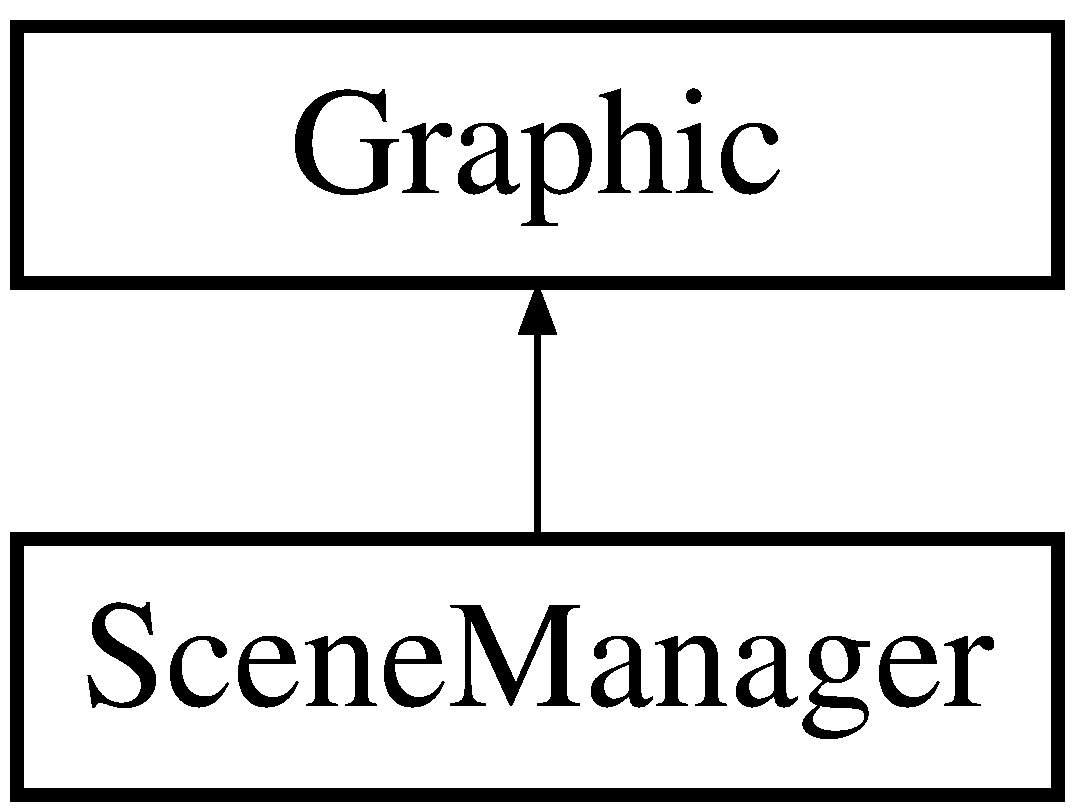
\includegraphics[height=2.000000cm]{class_scene_manager}
\end{center}
\end{figure}
\subsection*{Public Member Functions}
\begin{DoxyCompactItemize}
\item 
\mbox{\hyperlink{class_scene_manager_aeaf8d1701d0624f47f0274f2642154f2}{Scene\+Manager}} (unique\+\_\+ptr$<$ \mbox{\hyperlink{class_table}{Table}} $>$ table, vector$<$ unique\+\_\+ptr$<$ \mbox{\hyperlink{class_ball}{Ball}} $>$$>$ \&balls, bool f=false)
\begin{DoxyCompactList}\small\item\em \mbox{\hyperlink{class_scene_manager}{Scene\+Manager}} Constructor. \end{DoxyCompactList}\item 
void \mbox{\hyperlink{class_scene_manager_a1692dc970086f1cc481000da605c4628}{tick}} (float dtime)
\begin{DoxyCompactList}\small\item\em take a timestep of size dtime \end{DoxyCompactList}\item 
void \mbox{\hyperlink{class_scene_manager_a1acae2e8e78a37c3cb17c5d90a5882ca}{draw}} (Q\+Painter \&painter) const
\begin{DoxyCompactList}\small\item\em draw the current scene \end{DoxyCompactList}\item 
Q\+Size \mbox{\hyperlink{class_scene_manager_ad1c7f8a0c3e2e7d9211a442cd24253d4}{veiw\+Port}} () const
\begin{DoxyCompactList}\small\item\em retrives the size of the scene \end{DoxyCompactList}\item 
void \mbox{\hyperlink{class_scene_manager_a543db38edb424561aa3f0d845ed5c32a}{set\+Cue\+BallV}} (Q\+Vector2D vel)
\begin{DoxyCompactList}\small\item\em set the cue ball\textquotesingle{}s velocity \end{DoxyCompactList}\item 
void \mbox{\hyperlink{class_scene_manager_af7f98cdad994d8f8b982239ff54363da}{set\+Stage2\+Bool}} (bool f)
\begin{DoxyCompactList}\small\item\em set the bool member stage2 \end{DoxyCompactList}\item 
bool \mbox{\hyperlink{class_scene_manager_a425e6d6cae2f7f902027b8a8cba28d0a}{get\+Flag}} () const
\begin{DoxyCompactList}\small\item\em get the bool flag stage2 \end{DoxyCompactList}\item 
\mbox{\Hypertarget{class_scene_manager_acf825392b2abb023b088d9cae42849f0}\label{class_scene_manager_acf825392b2abb023b088d9cae42849f0}} 
void \mbox{\hyperlink{class_scene_manager_acf825392b2abb023b088d9cae42849f0}{reset\+BallV}} ()
\begin{DoxyCompactList}\small\item\em reset the ball\textquotesingle{}s velocity to zero, to prevent the ball doesnt stop with a really small vecolity \end{DoxyCompactList}\end{DoxyCompactItemize}


\subsection{Constructor \& Destructor Documentation}
\mbox{\Hypertarget{class_scene_manager_aeaf8d1701d0624f47f0274f2642154f2}\label{class_scene_manager_aeaf8d1701d0624f47f0274f2642154f2}} 
\index{Scene\+Manager@{Scene\+Manager}!Scene\+Manager@{Scene\+Manager}}
\index{Scene\+Manager@{Scene\+Manager}!Scene\+Manager@{Scene\+Manager}}
\subsubsection{\texorpdfstring{Scene\+Manager()}{SceneManager()}}
{\footnotesize\ttfamily Scene\+Manager\+::\+Scene\+Manager (\begin{DoxyParamCaption}\item[{unique\+\_\+ptr$<$ \mbox{\hyperlink{class_table}{Table}} $>$}]{table,  }\item[{vector$<$ unique\+\_\+ptr$<$ \mbox{\hyperlink{class_ball}{Ball}} $>$$>$ \&}]{balls,  }\item[{bool}]{f = {\ttfamily false} }\end{DoxyParamCaption})}



\mbox{\hyperlink{class_scene_manager}{Scene\+Manager}} Constructor. 


\begin{DoxyParams}{Parameters}
{\em table} & \\
\hline
{\em balls} & \\
\hline
\end{DoxyParams}


\subsection{Member Function Documentation}
\mbox{\Hypertarget{class_scene_manager_a1acae2e8e78a37c3cb17c5d90a5882ca}\label{class_scene_manager_a1acae2e8e78a37c3cb17c5d90a5882ca}} 
\index{Scene\+Manager@{Scene\+Manager}!draw@{draw}}
\index{draw@{draw}!Scene\+Manager@{Scene\+Manager}}
\subsubsection{\texorpdfstring{draw()}{draw()}}
{\footnotesize\ttfamily void Scene\+Manager\+::draw (\begin{DoxyParamCaption}\item[{Q\+Painter \&}]{painter }\end{DoxyParamCaption}) const\hspace{0.3cm}{\ttfamily [virtual]}}



draw the current scene 


\begin{DoxyParams}{Parameters}
{\em painter} & for rendering objects \\
\hline
\end{DoxyParams}


Implements \mbox{\hyperlink{class_graphic_aed0af75ae3756baeb3fe663ae5f36f29}{Graphic}}.

\mbox{\Hypertarget{class_scene_manager_a425e6d6cae2f7f902027b8a8cba28d0a}\label{class_scene_manager_a425e6d6cae2f7f902027b8a8cba28d0a}} 
\index{Scene\+Manager@{Scene\+Manager}!get\+Flag@{get\+Flag}}
\index{get\+Flag@{get\+Flag}!Scene\+Manager@{Scene\+Manager}}
\subsubsection{\texorpdfstring{get\+Flag()}{getFlag()}}
{\footnotesize\ttfamily bool Scene\+Manager\+::get\+Flag (\begin{DoxyParamCaption}{ }\end{DoxyParamCaption}) const}



get the bool flag stage2 

\begin{DoxyReturn}{Returns}
a bool type of stage2 
\end{DoxyReturn}
\mbox{\Hypertarget{class_scene_manager_a543db38edb424561aa3f0d845ed5c32a}\label{class_scene_manager_a543db38edb424561aa3f0d845ed5c32a}} 
\index{Scene\+Manager@{Scene\+Manager}!set\+Cue\+BallV@{set\+Cue\+BallV}}
\index{set\+Cue\+BallV@{set\+Cue\+BallV}!Scene\+Manager@{Scene\+Manager}}
\subsubsection{\texorpdfstring{set\+Cue\+Ball\+V()}{setCueBallV()}}
{\footnotesize\ttfamily void Scene\+Manager\+::set\+Cue\+BallV (\begin{DoxyParamCaption}\item[{Q\+Vector2D}]{vel }\end{DoxyParamCaption})}



set the cue ball\textquotesingle{}s velocity 


\begin{DoxyParams}{Parameters}
{\em the} & velocity \\
\hline
\end{DoxyParams}
\mbox{\Hypertarget{class_scene_manager_af7f98cdad994d8f8b982239ff54363da}\label{class_scene_manager_af7f98cdad994d8f8b982239ff54363da}} 
\index{Scene\+Manager@{Scene\+Manager}!set\+Stage2\+Bool@{set\+Stage2\+Bool}}
\index{set\+Stage2\+Bool@{set\+Stage2\+Bool}!Scene\+Manager@{Scene\+Manager}}
\subsubsection{\texorpdfstring{set\+Stage2\+Bool()}{setStage2Bool()}}
{\footnotesize\ttfamily void Scene\+Manager\+::set\+Stage2\+Bool (\begin{DoxyParamCaption}\item[{bool}]{f }\end{DoxyParamCaption})}



set the bool member stage2 


\begin{DoxyParams}{Parameters}
{\em a} & bool type named f \\
\hline
\end{DoxyParams}
\mbox{\Hypertarget{class_scene_manager_a1692dc970086f1cc481000da605c4628}\label{class_scene_manager_a1692dc970086f1cc481000da605c4628}} 
\index{Scene\+Manager@{Scene\+Manager}!tick@{tick}}
\index{tick@{tick}!Scene\+Manager@{Scene\+Manager}}
\subsubsection{\texorpdfstring{tick()}{tick()}}
{\footnotesize\ttfamily void Scene\+Manager\+::tick (\begin{DoxyParamCaption}\item[{float}]{dtime }\end{DoxyParamCaption})}



take a timestep of size dtime 


\begin{DoxyParams}{Parameters}
{\em dtime} & \\
\hline
\end{DoxyParams}
\mbox{\Hypertarget{class_scene_manager_ad1c7f8a0c3e2e7d9211a442cd24253d4}\label{class_scene_manager_ad1c7f8a0c3e2e7d9211a442cd24253d4}} 
\index{Scene\+Manager@{Scene\+Manager}!veiw\+Port@{veiw\+Port}}
\index{veiw\+Port@{veiw\+Port}!Scene\+Manager@{Scene\+Manager}}
\subsubsection{\texorpdfstring{veiw\+Port()}{veiwPort()}}
{\footnotesize\ttfamily Q\+Size Scene\+Manager\+::veiw\+Port (\begin{DoxyParamCaption}{ }\end{DoxyParamCaption}) const}



retrives the size of the scene 

\begin{DoxyReturn}{Returns}
the size of the scene 
\end{DoxyReturn}


The documentation for this class was generated from the following files\+:\begin{DoxyCompactItemize}
\item 
scenemanager.\+h\item 
scenemanager.\+cpp\end{DoxyCompactItemize}

\hypertarget{class_simple_ball}{}\section{Simple\+Ball Class Reference}
\label{class_simple_ball}\index{Simple\+Ball@{Simple\+Ball}}
Inheritance diagram for Simple\+Ball\+:\begin{figure}[H]
\begin{center}
\leavevmode
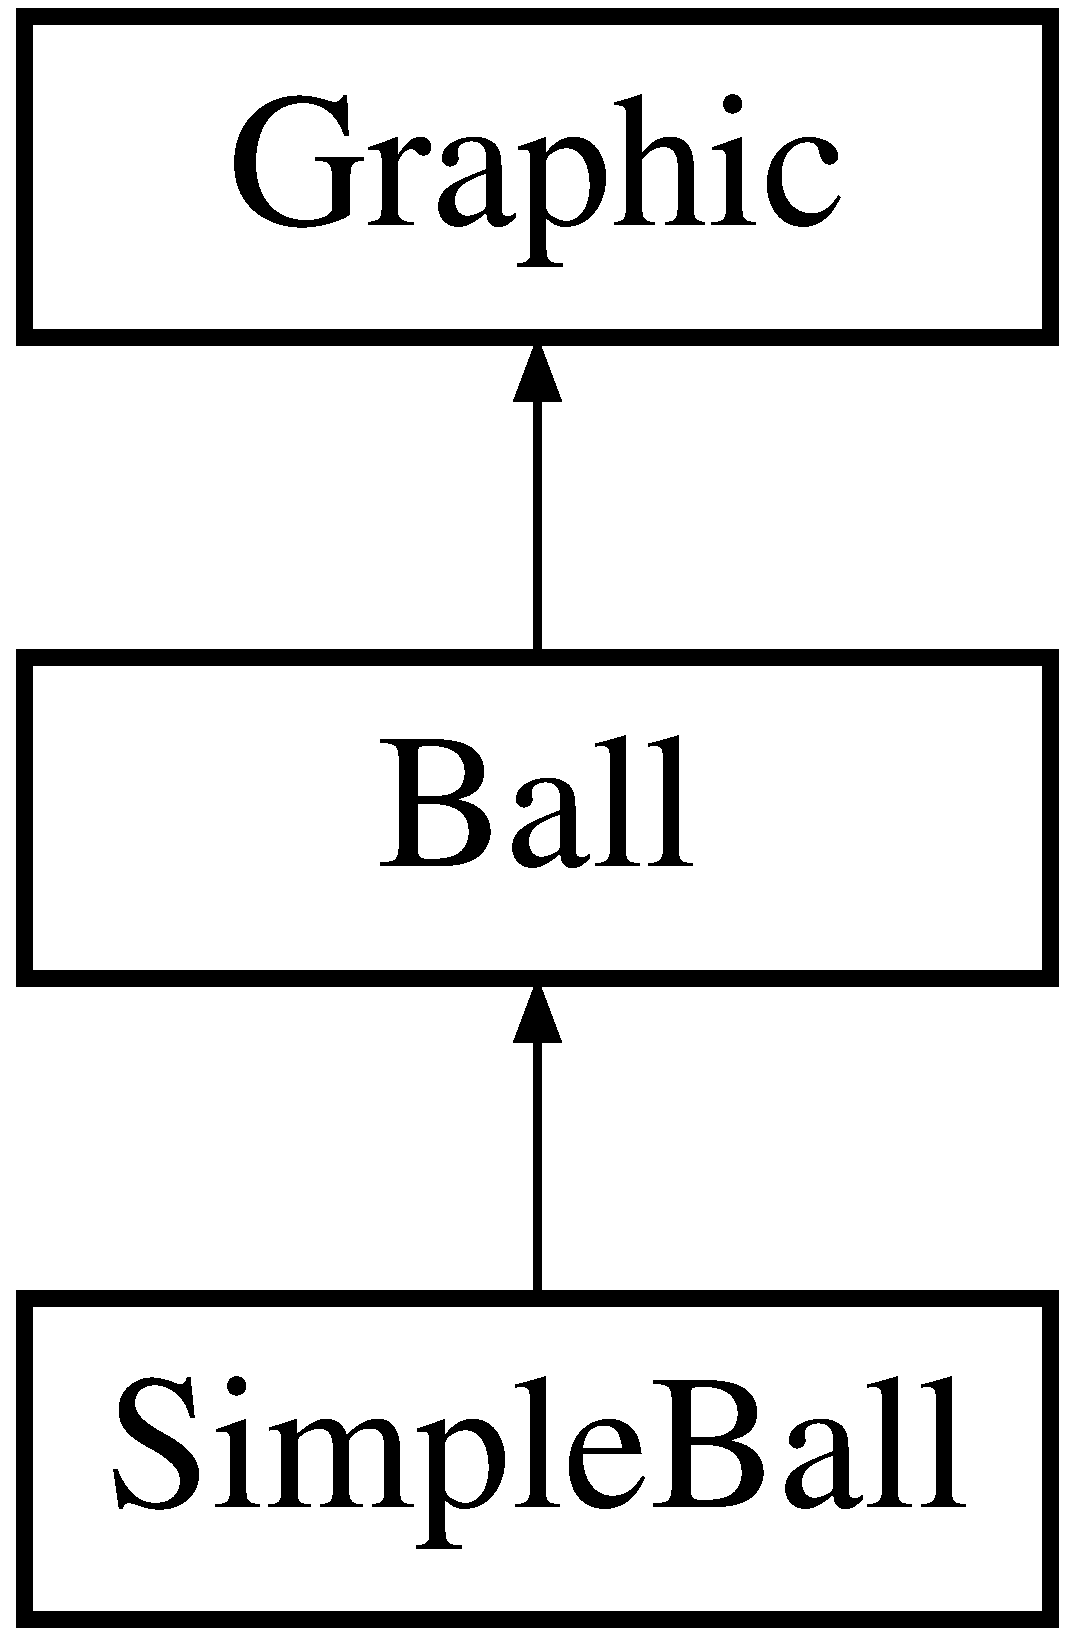
\includegraphics[height=3.000000cm]{class_simple_ball}
\end{center}
\end{figure}
\subsection*{Public Member Functions}
\begin{DoxyCompactItemize}
\item 
\mbox{\hyperlink{class_simple_ball_a73986d31758ab1201000aef11bef49aa}{Simple\+Ball}} (float radius=10, const Q\+Color \&color=Q\+Color(255, 255, 255), float mass=1.\+0, const Q\+Vector2D \&position=Q\+Vector2D(0, 0), const Q\+Vector2D \&velocity=Q\+Vector2D(0, 0), const double strength=std\+::numeric\+\_\+limits$<$ double $>$\+::max(), bool is\+Contained=false)
\begin{DoxyCompactList}\small\item\em \mbox{\hyperlink{class_simple_ball}{Simple\+Ball}} Constructor. \end{DoxyCompactList}\item 
void \mbox{\hyperlink{class_simple_ball_ad775dddec77276d6f92f8aea4b487df3}{draw}} (Q\+Painter \&painter) const override
\begin{DoxyCompactList}\small\item\em Draws the ball onto the scene. \end{DoxyCompactList}\item 
void \mbox{\hyperlink{class_simple_ball_a22ec99de5d096383f869a919f9f9abd7}{change\+Pfor\+Contained}} (const Q\+Vector2D \&delta) override
\begin{DoxyCompactList}\small\item\em change the position for contained balls. Inherited from base class, if no contained ball, then do nothing. \end{DoxyCompactList}\item 
float \mbox{\hyperlink{class_simple_ball_a0cb0b931a2e3fa9f2ffba6fd354985ea}{get\+Mass}} () const override
\begin{DoxyCompactList}\small\item\em get the mass of the ball \end{DoxyCompactList}\item 
double \mbox{\hyperlink{class_simple_ball_a3a4c5bc776e3788112f02320432ba8cc}{get\+Strength}} () const override
\begin{DoxyCompactList}\small\item\em get the strength of the ball \end{DoxyCompactList}\item 
int \mbox{\hyperlink{class_simple_ball_ac9c7e389cf03bfb2f3e71d66bf6608cd}{get\+Contained\+Ball\+Number}} () const override
\begin{DoxyCompactList}\small\item\em get the number of conatined ball \end{DoxyCompactList}\item 
void \mbox{\hyperlink{class_simple_ball_a5e100bd3bc3b700d3ce1c5028d95ac31}{change\+Vfor\+Contained}} (const Q\+Vector2D \&Parent\+Velocity, float energy\+Per\+Ball, const Q\+Vector2D \&point\+Of\+Collision) const override
\begin{DoxyCompactList}\small\item\em change the velocity for contained ball, inherited from base class, return 0 here \end{DoxyCompactList}\item 
void \mbox{\hyperlink{class_simple_ball_a1af03353f6c3414e6ce7c12a9b338e72}{move\+Out}} (std\+::vector$<$ unique\+\_\+ptr$<$ \mbox{\hyperlink{class_ball}{Ball}} $>$$>$ \&balls\+On\+Table) override
\begin{DoxyCompactList}\small\item\em move the contained balls out into given vector, inherited from base calss, do nothing here \end{DoxyCompactList}\item 
std\+::string \mbox{\hyperlink{class_simple_ball_aad4437558814bc8c6f276d5e09507eb4}{get\+Colour}} () const override
\begin{DoxyCompactList}\small\item\em get the colour of this ball \end{DoxyCompactList}\end{DoxyCompactItemize}
\subsection*{Additional Inherited Members}


\subsection{Constructor \& Destructor Documentation}
\mbox{\Hypertarget{class_simple_ball_a73986d31758ab1201000aef11bef49aa}\label{class_simple_ball_a73986d31758ab1201000aef11bef49aa}} 
\index{Simple\+Ball@{Simple\+Ball}!Simple\+Ball@{Simple\+Ball}}
\index{Simple\+Ball@{Simple\+Ball}!Simple\+Ball@{Simple\+Ball}}
\subsubsection{\texorpdfstring{Simple\+Ball()}{SimpleBall()}}
{\footnotesize\ttfamily Simple\+Ball\+::\+Simple\+Ball (\begin{DoxyParamCaption}\item[{float}]{radius = {\ttfamily 10},  }\item[{const Q\+Color \&}]{color = {\ttfamily QColor(255,~255,~255)},  }\item[{float}]{mass = {\ttfamily 1.0},  }\item[{const Q\+Vector2D \&}]{position = {\ttfamily QVector2D(0,~0)},  }\item[{const Q\+Vector2D \&}]{velocity = {\ttfamily QVector2D(0,~0)},  }\item[{const double}]{strength = {\ttfamily std\+:\+:numeric\+\_\+limits$<$double$>$\+:\+:max()},  }\item[{bool}]{is\+Contained = {\ttfamily false} }\end{DoxyParamCaption})}



\mbox{\hyperlink{class_simple_ball}{Simple\+Ball}} Constructor. 


\begin{DoxyParams}{Parameters}
{\em radius} & \\
\hline
{\em color} & \\
\hline
{\em mass} & \+: use 0 for infinite mass \\
\hline
{\em position} & \\
\hline
{\em velocity} & \\
\hline
\end{DoxyParams}


\subsection{Member Function Documentation}
\mbox{\Hypertarget{class_simple_ball_a22ec99de5d096383f869a919f9f9abd7}\label{class_simple_ball_a22ec99de5d096383f869a919f9f9abd7}} 
\index{Simple\+Ball@{Simple\+Ball}!change\+Pfor\+Contained@{change\+Pfor\+Contained}}
\index{change\+Pfor\+Contained@{change\+Pfor\+Contained}!Simple\+Ball@{Simple\+Ball}}
\subsubsection{\texorpdfstring{change\+Pfor\+Contained()}{changePforContained()}}
{\footnotesize\ttfamily void Simple\+Ball\+::change\+Pfor\+Contained (\begin{DoxyParamCaption}\item[{const Q\+Vector2D \&}]{delta }\end{DoxyParamCaption})\hspace{0.3cm}{\ttfamily [override]}, {\ttfamily [virtual]}}



change the position for contained balls. Inherited from base class, if no contained ball, then do nothing. 


\begin{DoxyParams}{Parameters}
{\em delta} & position \\
\hline
\end{DoxyParams}


Implements \mbox{\hyperlink{class_ball_a86aa99bb9b244c4ec9193f8ac09c6e8e}{Ball}}.

\mbox{\Hypertarget{class_simple_ball_a5e100bd3bc3b700d3ce1c5028d95ac31}\label{class_simple_ball_a5e100bd3bc3b700d3ce1c5028d95ac31}} 
\index{Simple\+Ball@{Simple\+Ball}!change\+Vfor\+Contained@{change\+Vfor\+Contained}}
\index{change\+Vfor\+Contained@{change\+Vfor\+Contained}!Simple\+Ball@{Simple\+Ball}}
\subsubsection{\texorpdfstring{change\+Vfor\+Contained()}{changeVforContained()}}
{\footnotesize\ttfamily void Simple\+Ball\+::change\+Vfor\+Contained (\begin{DoxyParamCaption}\item[{const Q\+Vector2D \&}]{Parent\+Velocity,  }\item[{float}]{energy\+Per\+Ball,  }\item[{const Q\+Vector2D \&}]{point\+Of\+Collision }\end{DoxyParamCaption}) const\hspace{0.3cm}{\ttfamily [override]}, {\ttfamily [virtual]}}



change the velocity for contained ball, inherited from base class, return 0 here 


\begin{DoxyParams}{Parameters}
{\em parent\textquotesingle{}s} & velocity \\
\hline
{\em engergy} & gained by collison \\
\hline
{\em the} & point of collision \\
\hline
\end{DoxyParams}


Implements \mbox{\hyperlink{class_ball_a43cfbf4dca89a94048b4d45b2eaf62e9}{Ball}}.

\mbox{\Hypertarget{class_simple_ball_ad775dddec77276d6f92f8aea4b487df3}\label{class_simple_ball_ad775dddec77276d6f92f8aea4b487df3}} 
\index{Simple\+Ball@{Simple\+Ball}!draw@{draw}}
\index{draw@{draw}!Simple\+Ball@{Simple\+Ball}}
\subsubsection{\texorpdfstring{draw()}{draw()}}
{\footnotesize\ttfamily void Simple\+Ball\+::draw (\begin{DoxyParamCaption}\item[{Q\+Painter \&}]{painter }\end{DoxyParamCaption}) const\hspace{0.3cm}{\ttfamily [override]}, {\ttfamily [virtual]}}



Draws the ball onto the scene. 


\begin{DoxyParams}{Parameters}
{\em painter} & for rendering the ball \\
\hline
\end{DoxyParams}


Implements \mbox{\hyperlink{class_graphic_aed0af75ae3756baeb3fe663ae5f36f29}{Graphic}}.

\mbox{\Hypertarget{class_simple_ball_aad4437558814bc8c6f276d5e09507eb4}\label{class_simple_ball_aad4437558814bc8c6f276d5e09507eb4}} 
\index{Simple\+Ball@{Simple\+Ball}!get\+Colour@{get\+Colour}}
\index{get\+Colour@{get\+Colour}!Simple\+Ball@{Simple\+Ball}}
\subsubsection{\texorpdfstring{get\+Colour()}{getColour()}}
{\footnotesize\ttfamily std\+::string Simple\+Ball\+::get\+Colour (\begin{DoxyParamCaption}{ }\end{DoxyParamCaption}) const\hspace{0.3cm}{\ttfamily [override]}, {\ttfamily [virtual]}}



get the colour of this ball 

\begin{DoxyReturn}{Returns}
a string type of name of the colour 
\end{DoxyReturn}


Implements \mbox{\hyperlink{class_ball_a248c8a5fc9b8770840f275ea7057b012}{Ball}}.

\mbox{\Hypertarget{class_simple_ball_ac9c7e389cf03bfb2f3e71d66bf6608cd}\label{class_simple_ball_ac9c7e389cf03bfb2f3e71d66bf6608cd}} 
\index{Simple\+Ball@{Simple\+Ball}!get\+Contained\+Ball\+Number@{get\+Contained\+Ball\+Number}}
\index{get\+Contained\+Ball\+Number@{get\+Contained\+Ball\+Number}!Simple\+Ball@{Simple\+Ball}}
\subsubsection{\texorpdfstring{get\+Contained\+Ball\+Number()}{getContainedBallNumber()}}
{\footnotesize\ttfamily int Simple\+Ball\+::get\+Contained\+Ball\+Number (\begin{DoxyParamCaption}{ }\end{DoxyParamCaption}) const\hspace{0.3cm}{\ttfamily [override]}, {\ttfamily [virtual]}}



get the number of conatined ball 

\begin{DoxyReturn}{Returns}
return the integer of ball number 
\end{DoxyReturn}


Implements \mbox{\hyperlink{class_ball_a13794c8d0e0863301a5f321a617542f6}{Ball}}.

\mbox{\Hypertarget{class_simple_ball_a0cb0b931a2e3fa9f2ffba6fd354985ea}\label{class_simple_ball_a0cb0b931a2e3fa9f2ffba6fd354985ea}} 
\index{Simple\+Ball@{Simple\+Ball}!get\+Mass@{get\+Mass}}
\index{get\+Mass@{get\+Mass}!Simple\+Ball@{Simple\+Ball}}
\subsubsection{\texorpdfstring{get\+Mass()}{getMass()}}
{\footnotesize\ttfamily float Simple\+Ball\+::get\+Mass (\begin{DoxyParamCaption}{ }\end{DoxyParamCaption}) const\hspace{0.3cm}{\ttfamily [override]}, {\ttfamily [virtual]}}



get the mass of the ball 

\begin{DoxyReturn}{Returns}
a float type of mass 
\end{DoxyReturn}


Implements \mbox{\hyperlink{class_ball_ab755ce741a2f0b652f499d183376be04}{Ball}}.

\mbox{\Hypertarget{class_simple_ball_a3a4c5bc776e3788112f02320432ba8cc}\label{class_simple_ball_a3a4c5bc776e3788112f02320432ba8cc}} 
\index{Simple\+Ball@{Simple\+Ball}!get\+Strength@{get\+Strength}}
\index{get\+Strength@{get\+Strength}!Simple\+Ball@{Simple\+Ball}}
\subsubsection{\texorpdfstring{get\+Strength()}{getStrength()}}
{\footnotesize\ttfamily double Simple\+Ball\+::get\+Strength (\begin{DoxyParamCaption}{ }\end{DoxyParamCaption}) const\hspace{0.3cm}{\ttfamily [override]}, {\ttfamily [virtual]}}



get the strength of the ball 

\begin{DoxyReturn}{Returns}
a double type of strength 
\end{DoxyReturn}


Implements \mbox{\hyperlink{class_ball_ab659c8dceb67abdd09423814d4fc879e}{Ball}}.

\mbox{\Hypertarget{class_simple_ball_a1af03353f6c3414e6ce7c12a9b338e72}\label{class_simple_ball_a1af03353f6c3414e6ce7c12a9b338e72}} 
\index{Simple\+Ball@{Simple\+Ball}!move\+Out@{move\+Out}}
\index{move\+Out@{move\+Out}!Simple\+Ball@{Simple\+Ball}}
\subsubsection{\texorpdfstring{move\+Out()}{moveOut()}}
{\footnotesize\ttfamily void Simple\+Ball\+::move\+Out (\begin{DoxyParamCaption}\item[{std\+::vector$<$ unique\+\_\+ptr$<$ \mbox{\hyperlink{class_ball}{Ball}} $>$$>$ \&}]{balls\+On\+Table }\end{DoxyParamCaption})\hspace{0.3cm}{\ttfamily [override]}, {\ttfamily [virtual]}}



move the contained balls out into given vector, inherited from base calss, do nothing here 


\begin{DoxyParams}{Parameters}
{\em the} & given vector for new balls \\
\hline
\end{DoxyParams}


Implements \mbox{\hyperlink{class_ball_a7d3b8c70ee8c61db73692a4d44bbf933}{Ball}}.



The documentation for this class was generated from the following files\+:\begin{DoxyCompactItemize}
\item 
simpleball.\+h\item 
simpleball.\+cpp\end{DoxyCompactItemize}

\hypertarget{class_simple_creator}{}\section{Simple\+Creator Class Reference}
\label{class_simple_creator}\index{Simple\+Creator@{Simple\+Creator}}
Inheritance diagram for Simple\+Creator\+:\begin{figure}[H]
\begin{center}
\leavevmode
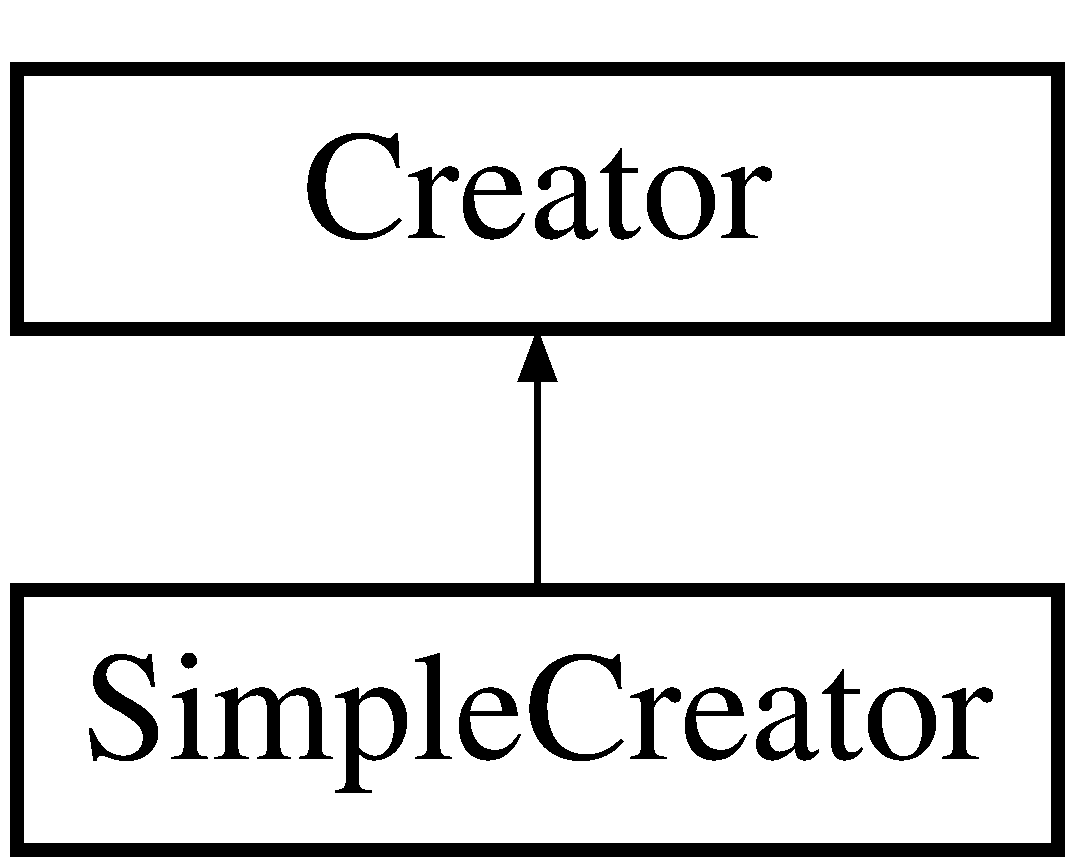
\includegraphics[height=2.000000cm]{class_simple_creator}
\end{center}
\end{figure}
\subsection*{Protected Member Functions}
\begin{DoxyCompactItemize}
\item 
unique\+\_\+ptr$<$ \mbox{\hyperlink{class_table}{Table}} $>$ \mbox{\hyperlink{class_simple_creator_af6556afca4e573deaaf624e8be14dfae}{make\+Table}} (const Q\+Json\+Object \&spec, int f=1)
\begin{DoxyCompactList}\small\item\em makes a \mbox{\hyperlink{class_simple_table}{Simple\+Table}} from J\+S\+ON config \end{DoxyCompactList}\item 
unique\+\_\+ptr$<$ \mbox{\hyperlink{class_ball}{Ball}} $>$ \mbox{\hyperlink{class_simple_creator_a8e5fdfc8bcd5a661cdcfb49d33a51910}{make\+Ball}} (const Q\+Json\+Object \&spec, int f=1)
\begin{DoxyCompactList}\small\item\em makes a \mbox{\hyperlink{class_simple_ball}{Simple\+Ball}} from the J\+S\+ON config \end{DoxyCompactList}\item 
unique\+\_\+ptr$<$ \mbox{\hyperlink{class_ball}{Ball}} $>$ \mbox{\hyperlink{class_simple_creator_a7fdf1b117c73c93da53694639ff6fc6c}{make\+Contained\+Ball}} (const Q\+Json\+Object \&spec, const Q\+Color \&colour, const Q\+Vector2D \&position)
\begin{DoxyCompactList}\small\item\em make contained ball, can be in a recursive way \end{DoxyCompactList}\end{DoxyCompactItemize}
\subsection*{Protected Attributes}
\begin{DoxyCompactItemize}
\item 
\mbox{\Hypertarget{class_simple_creator_a7645d79be8e3c339826bb8fe585dbabb}\label{class_simple_creator_a7645d79be8e3c339826bb8fe585dbabb}} 
float {\bfseries table\+Height}
\item 
\mbox{\Hypertarget{class_simple_creator_aac38f49aba11104b8424df0867174e0c}\label{class_simple_creator_aac38f49aba11104b8424df0867174e0c}} 
float {\bfseries table\+Width}
\end{DoxyCompactItemize}
\subsection*{Additional Inherited Members}


\subsection{Member Function Documentation}
\mbox{\Hypertarget{class_simple_creator_a8e5fdfc8bcd5a661cdcfb49d33a51910}\label{class_simple_creator_a8e5fdfc8bcd5a661cdcfb49d33a51910}} 
\index{Simple\+Creator@{Simple\+Creator}!make\+Ball@{make\+Ball}}
\index{make\+Ball@{make\+Ball}!Simple\+Creator@{Simple\+Creator}}
\subsubsection{\texorpdfstring{make\+Ball()}{makeBall()}}
{\footnotesize\ttfamily unique\+\_\+ptr$<$ \mbox{\hyperlink{class_ball}{Ball}} $>$ Simple\+Creator\+::make\+Ball (\begin{DoxyParamCaption}\item[{const Q\+Json\+Object \&}]{spec,  }\item[{int}]{f = {\ttfamily 1} }\end{DoxyParamCaption})\hspace{0.3cm}{\ttfamily [protected]}, {\ttfamily [virtual]}}



makes a \mbox{\hyperlink{class_simple_ball}{Simple\+Ball}} from the J\+S\+ON config 


\begin{DoxyParams}{Parameters}
{\em spec} & a J\+S\+ON configuration for the ball\\
\hline
\end{DoxyParams}
\begin{DoxyReturn}{Returns}
a \mbox{\hyperlink{class_simple_ball}{Simple\+Ball}} with the specified configuration 
\end{DoxyReturn}


Implements \mbox{\hyperlink{class_creator_aa3f6415656f52625d4f3051bfa70d4eb}{Creator}}.

\mbox{\Hypertarget{class_simple_creator_a7fdf1b117c73c93da53694639ff6fc6c}\label{class_simple_creator_a7fdf1b117c73c93da53694639ff6fc6c}} 
\index{Simple\+Creator@{Simple\+Creator}!make\+Contained\+Ball@{make\+Contained\+Ball}}
\index{make\+Contained\+Ball@{make\+Contained\+Ball}!Simple\+Creator@{Simple\+Creator}}
\subsubsection{\texorpdfstring{make\+Contained\+Ball()}{makeContainedBall()}}
{\footnotesize\ttfamily unique\+\_\+ptr$<$ \mbox{\hyperlink{class_ball}{Ball}} $>$ Simple\+Creator\+::make\+Contained\+Ball (\begin{DoxyParamCaption}\item[{const Q\+Json\+Object \&}]{spec,  }\item[{const Q\+Color \&}]{colour,  }\item[{const Q\+Vector2D \&}]{position }\end{DoxyParamCaption})\hspace{0.3cm}{\ttfamily [protected]}}



make contained ball, can be in a recursive way 


\begin{DoxyParams}{Parameters}
{\em Q\+Json\+Object} & to get config information from json file \\
\hline
{\em the} & colour from its mother ball for default use \\
\hline
{\em the} & position from its mother ball\\
\hline
\end{DoxyParams}
\begin{DoxyReturn}{Returns}
a contained ball with the specified configuration 
\end{DoxyReturn}
\mbox{\Hypertarget{class_simple_creator_af6556afca4e573deaaf624e8be14dfae}\label{class_simple_creator_af6556afca4e573deaaf624e8be14dfae}} 
\index{Simple\+Creator@{Simple\+Creator}!make\+Table@{make\+Table}}
\index{make\+Table@{make\+Table}!Simple\+Creator@{Simple\+Creator}}
\subsubsection{\texorpdfstring{make\+Table()}{makeTable()}}
{\footnotesize\ttfamily unique\+\_\+ptr$<$ \mbox{\hyperlink{class_table}{Table}} $>$ Simple\+Creator\+::make\+Table (\begin{DoxyParamCaption}\item[{const Q\+Json\+Object \&}]{spec,  }\item[{int}]{f = {\ttfamily 1} }\end{DoxyParamCaption})\hspace{0.3cm}{\ttfamily [protected]}, {\ttfamily [virtual]}}



makes a \mbox{\hyperlink{class_simple_table}{Simple\+Table}} from J\+S\+ON config 


\begin{DoxyParams}{Parameters}
{\em spec} & a J\+S\+ON configuration for the table\\
\hline
\end{DoxyParams}
\begin{DoxyReturn}{Returns}
a \mbox{\hyperlink{class_simple_table}{Simple\+Table}} with the specified configuration 
\end{DoxyReturn}


Implements \mbox{\hyperlink{class_creator_a70c571c0b776a5f29494f660957e0710}{Creator}}.



The documentation for this class was generated from the following files\+:\begin{DoxyCompactItemize}
\item 
simplecreator.\+h\item 
simplecreator.\+cpp\end{DoxyCompactItemize}

\hypertarget{class_simple_table}{}\section{Simple\+Table Class Reference}
\label{class_simple_table}\index{Simple\+Table@{Simple\+Table}}
Inheritance diagram for Simple\+Table\+:\begin{figure}[H]
\begin{center}
\leavevmode
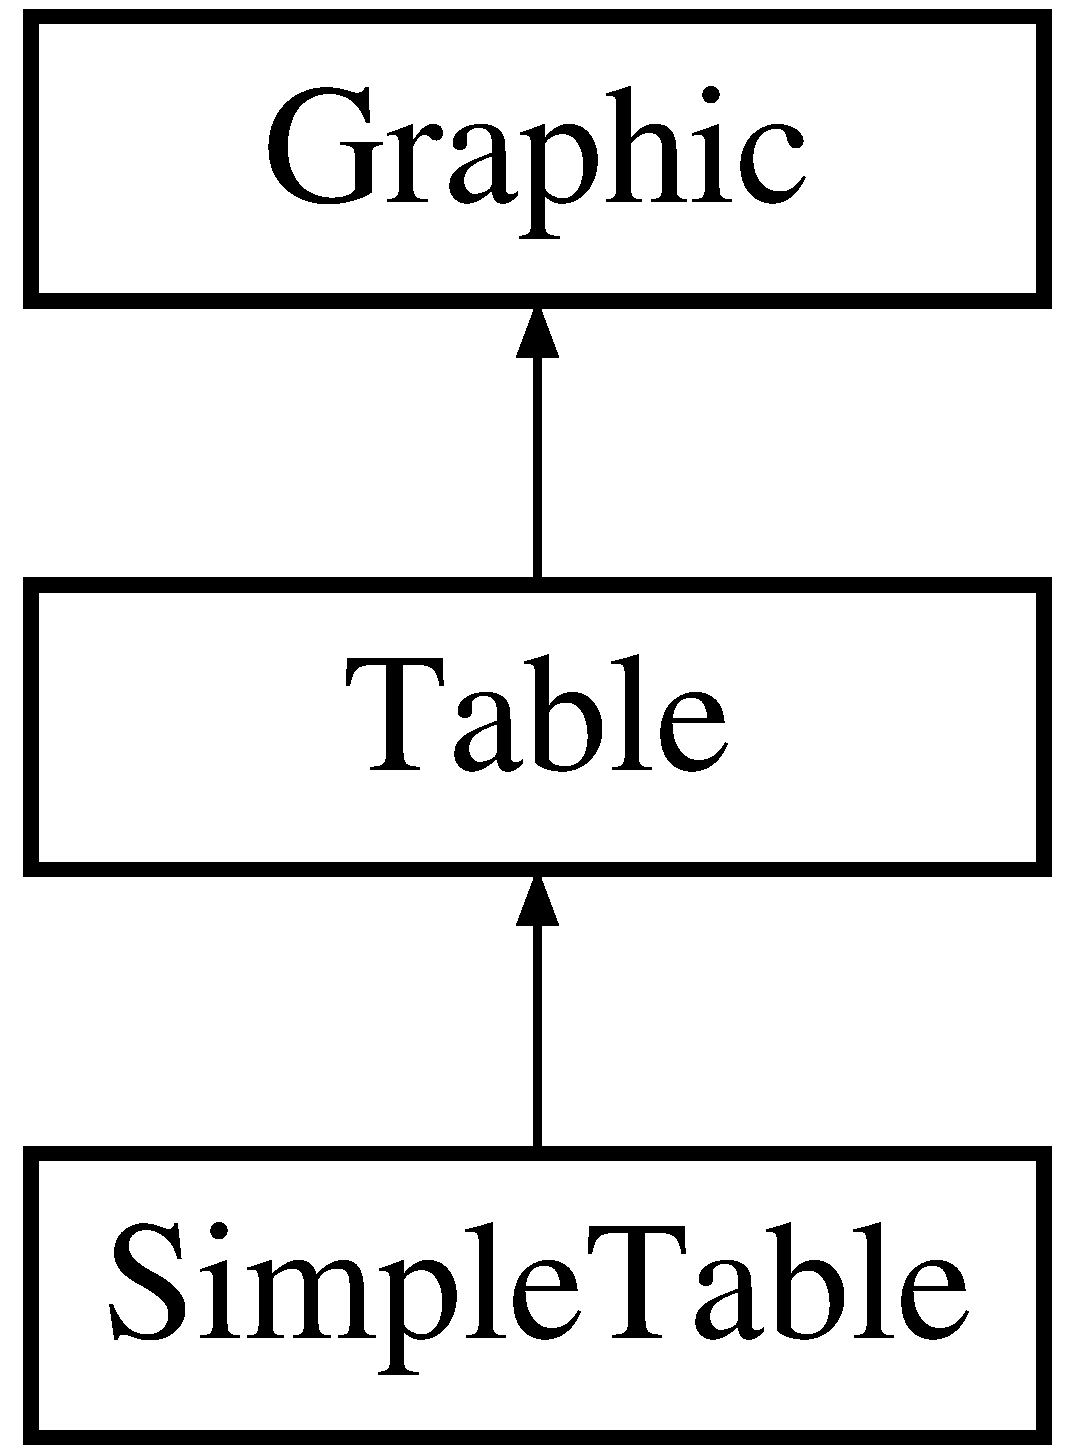
\includegraphics[height=3.000000cm]{class_simple_table}
\end{center}
\end{figure}
\subsection*{Public Member Functions}
\begin{DoxyCompactItemize}
\item 
\mbox{\hyperlink{class_simple_table_a18bc58d5eb57cafc2e4121d034605c1b}{Simple\+Table}} (const Q\+Size \&dim, const Q\+Color \&color, float friction, vector$<$ unique\+\_\+ptr$<$ \mbox{\hyperlink{class_pocket}{Pocket}} $>$$>$ \&pockets)
\begin{DoxyCompactList}\small\item\em \mbox{\hyperlink{class_simple_table}{Simple\+Table}} constructor. \end{DoxyCompactList}\item 
void \mbox{\hyperlink{class_simple_table_aabb9fe0665f1145ba620c1f6ff9b5576}{draw}} (Q\+Painter \&painter) const
\begin{DoxyCompactList}\small\item\em Draws the table onto the scene. \end{DoxyCompactList}\end{DoxyCompactItemize}
\subsection*{Public Attributes}
\begin{DoxyCompactItemize}
\item 
\mbox{\Hypertarget{class_simple_table_abe867fd6335990b297fe0b2e57154e06}\label{class_simple_table_abe867fd6335990b297fe0b2e57154e06}} 
Q\+Color {\bfseries color}
\end{DoxyCompactItemize}


\subsection{Constructor \& Destructor Documentation}
\mbox{\Hypertarget{class_simple_table_a18bc58d5eb57cafc2e4121d034605c1b}\label{class_simple_table_a18bc58d5eb57cafc2e4121d034605c1b}} 
\index{Simple\+Table@{Simple\+Table}!Simple\+Table@{Simple\+Table}}
\index{Simple\+Table@{Simple\+Table}!Simple\+Table@{Simple\+Table}}
\subsubsection{\texorpdfstring{Simple\+Table()}{SimpleTable()}}
{\footnotesize\ttfamily Simple\+Table\+::\+Simple\+Table (\begin{DoxyParamCaption}\item[{const Q\+Size \&}]{dim,  }\item[{const Q\+Color \&}]{color,  }\item[{float}]{friction,  }\item[{vector$<$ unique\+\_\+ptr$<$ \mbox{\hyperlink{class_pocket}{Pocket}} $>$$>$ \&}]{pockets }\end{DoxyParamCaption})}



\mbox{\hyperlink{class_simple_table}{Simple\+Table}} constructor. 


\begin{DoxyParams}{Parameters}
{\em dimension} & \+: size of the table \\
\hline
{\em color} & \\
\hline
{\em friction} & \\
\hline
\end{DoxyParams}


\subsection{Member Function Documentation}
\mbox{\Hypertarget{class_simple_table_aabb9fe0665f1145ba620c1f6ff9b5576}\label{class_simple_table_aabb9fe0665f1145ba620c1f6ff9b5576}} 
\index{Simple\+Table@{Simple\+Table}!draw@{draw}}
\index{draw@{draw}!Simple\+Table@{Simple\+Table}}
\subsubsection{\texorpdfstring{draw()}{draw()}}
{\footnotesize\ttfamily void Simple\+Table\+::draw (\begin{DoxyParamCaption}\item[{Q\+Painter \&}]{painter }\end{DoxyParamCaption}) const\hspace{0.3cm}{\ttfamily [virtual]}}



Draws the table onto the scene. 


\begin{DoxyParams}{Parameters}
{\em painter} & for rendering the table \\
\hline
\end{DoxyParams}


Implements \mbox{\hyperlink{class_graphic_aed0af75ae3756baeb3fe663ae5f36f29}{Graphic}}.



The documentation for this class was generated from the following files\+:\begin{DoxyCompactItemize}
\item 
simpletable.\+h\item 
simpletable.\+cpp\end{DoxyCompactItemize}

\hypertarget{class_table}{}\section{Table Class Reference}
\label{class_table}\index{Table@{Table}}
Inheritance diagram for Table\+:\begin{figure}[H]
\begin{center}
\leavevmode
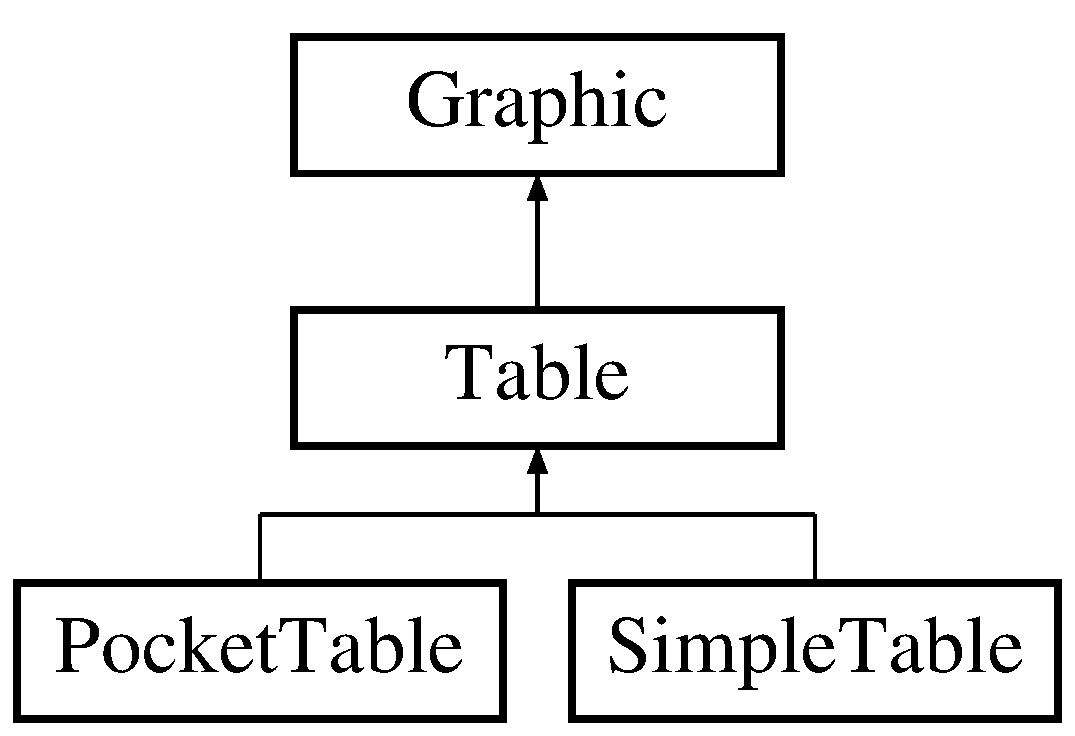
\includegraphics[height=3.000000cm]{class_table}
\end{center}
\end{figure}
\subsection*{Public Member Functions}
\begin{DoxyCompactItemize}
\item 
\mbox{\hyperlink{class_table_aa12fd8e1655bfdf20ba5bfbe7e6c9b0f}{Table}} (const Q\+Size \&dimension, float friction, vector$<$ unique\+\_\+ptr$<$ \mbox{\hyperlink{class_pocket}{Pocket}} $>$$>$ \&pockets)
\begin{DoxyCompactList}\small\item\em Constructor for \mbox{\hyperlink{class_table}{Table}}. \end{DoxyCompactList}\end{DoxyCompactItemize}
\subsection*{Public Attributes}
\begin{DoxyCompactItemize}
\item 
\mbox{\Hypertarget{class_table_a7b1a7786abc4b144d7f2e6c1a82fff21}\label{class_table_a7b1a7786abc4b144d7f2e6c1a82fff21}} 
Q\+Size {\bfseries dimension}
\item 
\mbox{\Hypertarget{class_table_ad14cbe09cafee32b3fb47df06827c91e}\label{class_table_ad14cbe09cafee32b3fb47df06827c91e}} 
float {\bfseries surface\+\_\+friction}
\item 
\mbox{\Hypertarget{class_table_abd8df756961b9e74d8986e5c50cdfd4e}\label{class_table_abd8df756961b9e74d8986e5c50cdfd4e}} 
vector$<$ unique\+\_\+ptr$<$ \mbox{\hyperlink{class_pocket}{Pocket}} $>$ $>$ {\bfseries pockets}
\end{DoxyCompactItemize}


\subsection{Constructor \& Destructor Documentation}
\mbox{\Hypertarget{class_table_aa12fd8e1655bfdf20ba5bfbe7e6c9b0f}\label{class_table_aa12fd8e1655bfdf20ba5bfbe7e6c9b0f}} 
\index{Table@{Table}!Table@{Table}}
\index{Table@{Table}!Table@{Table}}
\subsubsection{\texorpdfstring{Table()}{Table()}}
{\footnotesize\ttfamily Table\+::\+Table (\begin{DoxyParamCaption}\item[{const Q\+Size \&}]{dimension,  }\item[{float}]{friction,  }\item[{vector$<$ unique\+\_\+ptr$<$ \mbox{\hyperlink{class_pocket}{Pocket}} $>$$>$ \&}]{pockets }\end{DoxyParamCaption})\hspace{0.3cm}{\ttfamily [inline]}}



Constructor for \mbox{\hyperlink{class_table}{Table}}. 


\begin{DoxyParams}{Parameters}
{\em dimension} & \\
\hline
{\em friction} & \\
\hline
\end{DoxyParams}


The documentation for this class was generated from the following file\+:\begin{DoxyCompactItemize}
\item 
table.\+h\end{DoxyCompactItemize}

%--- End generated contents ---

% Index
\backmatter
\newpage
\phantomsection
\clearemptydoublepage
\addcontentsline{toc}{chapter}{Index}
\printindex

\end{document}
